\documentclass[12pt,a4paper]{report}

%==============================================================================
% PREAMBLE AND PACKAGES (Aligned with CEK / KTU B.Tech Project Format)
%==============================================================================
\usepackage{graphicx}
\usepackage{amsmath}
\usepackage{fancyhdr}
\usepackage{cite}
\usepackage{a4wide}
\usepackage{float}
\usepackage{epsfig}
\usepackage{longtable}
\usepackage{enumerate}
\usepackage{afterpage}
\usepackage{multirow}
\usepackage{ragged2e}
\usepackage{gensymb}
\usepackage{amsfonts} 
\usepackage[left=3.5cm,top=1.5cm,right=3cm,bottom=3cm]{geometry}
\usepackage{setspace}           
\usepackage{txfonts}
\usepackage{tikz}
\usetikzlibrary{calc, shapes.geometric, arrows, arrows.meta, positioning, fit, backgrounds, shadows}
\usepackage{subfiles}
\usepackage{adjustbox}
\usepackage{tcolorbox}
\tcbuselibrary{skins}

\newcommand{\Usefont}[1]{\fontfamily{#1}\selectfont}

\usepackage{lscape}
\linespread{1.5}

\usepackage{url}
\usepackage{subcaption}
\usepackage[intoc, english]{nomencl}
\usepackage[nottoc]{tocbibind}
\usepackage{booktabs}
\usepackage{array}
\usepackage{tabularx}
\usepackage{hyperref}

\hypersetup{
    plainpages=false,
    pdfpagelabels=true,
    colorlinks=true,
    linkcolor=black,
    citecolor=black,
    urlcolor=black,
    pdftitle={PrismSpace: An Intelligent Developer Operating Environment and Multi-Agent Orchestration Platform},
    pdfauthor={Group 01: Nobin Sijo, Pranav P, Prasanth P, Sankar Narayan S}
}

% Robust spacing and line-breaking settings to prevent overflow and overfull hboxes
\setlength{\headheight}{15pt}
\hyphenpenalty=1000
\tolerance=2000
\emergencystretch=2.5em

\bibliographystyle{IEEEtran}
\renewcommand{\bibname}{References}

% Figure search path
\graphicspath{{figures/}{diagrams/}{./}}

%==============================================================================
% METADATA DEFINITIONS (Project Group 01 & CEK)
%==============================================================================
\gdef \title{PRISMSPACE: AN INTELLIGENT DEVELOPER OPERATING ENVIRONMENT AND MULTI-AGENT ORCHESTRATION PLATFORM}
\gdef \shorttitle{PrismSpace: Intelligent Multi-Agent Platform}

\gdef \authorA{NOBIN SIJO}
\gdef \rollnoA{KNP23CS082}

\gdef \authorB{PRANAV P}
\gdef \rollnoB{KNP23CS085}

\gdef \authorC{PRASANTH P}
\gdef \rollnoC{KNP23CS086}

\gdef \authorD{SANKAR NARAYAN S}
\gdef \rollnoD{KNP23CS094}

\gdef \acadyear{2026--2027}
\gdef \submonth{October 2026}
\gdef \month{October 2026}
\gdef \date{28-10-2026}
\gdef \dept{Computer Science and Engineering}
\gdef \deptabbr{Dept. of CSE}
\gdef \degree{Bachelor of Technology}
\gdef \branch{Computer Science and Engineering}
\gdef \college{College of Engineering Karunagappally}
\gdef \collegeplace{Kollam}
\gdef \collegetown{Karunagappally}

\gdef \guide{Dr. Leena Silvoster}
\gdef \guidedes{Associate Professor}
\gdef \hod{Dr. Smitha P}
\gdef \hoddes{Professor and Head}

%==============================================================================
% DOCUMENT BODY
%==============================================================================
\begin{document}

%------------------------------------------------------------------------------
% FRONT MATTER
%------------------------------------------------------------------------------
\hypersetup{pageanchor=false}
%==================================coverpage.tex================================

\thispagestyle{empty}
\begin{titlepage}
\subfile{design_cover}
	\begin{center}\fontfamily{ptm}\selectfont
		{\Large \bfseries \title \par}
		\vspace*{12pt}
		{\large \Usefont{pzc}
			A PROJECT REPORT \par
			\vspace*{5pt}
			Submitted to the APJ Abdul Kalam Technological University \par
			\vspace*{5pt}
			in partial fulfillment of requirements for the award of degree\par}
		\vspace*{8pt}
		{\large \bfseries Bachelor of Technology}\par
		{\large in}\par
		{\large \bfseries \branch}\par
		\vspace*{10pt}
		{\large by}\par
		\vspace*{6pt}
		\begin{tabular}{c@{\hspace{2.2cm}}c}
			\large\bfseries NOBIN SIJO & \large\bfseries KNP23CS082 \\
			\large\bfseries PRANAV P & \large\bfseries KNP23CS085 \\
			\large\bfseries PRASANTH P & \large\bfseries KNP23CS086 \\
			\large\bfseries SANKAR NARAYAN S & \large\bfseries KNP23CS094
		\end{tabular}\par
		\vspace*{14pt}
		{
\includegraphics[width=4.0cm]{cek-logo.png}}\par
		\vspace{\stretch{0.5}}
		{\small \bfseries DEPARTMENT OF COMPUTER SCIENCE AND ENGINEERING}\par
		\vspace*{4pt}
		{\bfseries COLLEGE OF ENGINEERING KARUNAGAPPALLY}\par
		\vspace*{4pt}
		{\bfseries KOLLAM, KERALA}\par
		\vspace*{4pt}
		{\bfseries \submonth}\par
	\end{center}
\end{titlepage}

%==================================certificate1.tex================================
% Certificate page for B.Tech Project Report Group 01

\newpage
\thispagestyle{empty}

\begin{spacing}{1.18}

\begin{center}
	\textbf{DEPARTMENT OF COMPUTER SCIENCE AND ENGINEERING}\\
	\textbf{COLLEGE OF ENGINEERING KARUNAGAPPALLY}\\
	\vspace*{3pt}
	\textbf{\acadyear}
\end{center}

\vspace*{6pt}
\begin{center}
	
\includegraphics[width=3.6cm]{cek-logo.png}
\end{center}

\vspace*{6pt}
\begin{center}
	\textbf{\Large CERTIFICATE}
\end{center}
\vspace*{8pt}

\noindent This is to certify that the report entitled \textbf{\title} submitted by \textbf{NOBIN~SIJO} (\rollnoA), \textbf{PRANAV~P} (\rollnoB), \textbf{PRASANTH~P} (\rollnoC), and \textbf{SANKAR~NARAYAN~S} (\rollnoD), to the Department of \branch\ in partial fulfillment of the requirements for the award of the degree of Bachelor of Technology in \textbf{\branch}\ of the APJ Abdul Kalam Technological University is a bonafide record of the project work carried out by them under our guidance and supervision. This report in any form has not been submitted to any other University or Institute for any purpose.

\vspace*{1.0cm}

	\noindent\begin{minipage}[t]{0.48\textwidth}
		\raggedright
		\textbf{\guide} \\
		(Project Guide) \\
		\guidedes \\
		\deptabbr \\
		College of Engineering \\
		\collegetown
	\end{minipage}%
	\hfill
	\begin{minipage}[t]{0.48\textwidth}
		\raggedright
		\textbf{\coordinator} \\
		(Project Coordinator) \\
		\coordinatordes \\
		\deptabbr \\
		College of Engineering \\
		\collegetown
	\end{minipage}

	\vspace*{0.9cm}

	\begin{center}
		\textbf{\hod} \\
		\hoddes \\
		\deptabbr \\
		College of Engineering \\
		\collegetown
	\end{center}

\end{spacing}

\thispagestyle{empty}
%============================================================================

%==================================declaration.tex================================
\newpage
\thispagestyle{empty}

\begin{center}
\vspace*{20pt}
\textbf{\large DECLARATION}\\[16pt]
\end{center}

\noindent We, \textbf{NOBIN~SIJO} (\rollnoA), \textbf{PRANAV~P} (\rollnoB), \textbf{PRASANTH~P} (\rollnoC), and \textbf{SANKAR~NARAYAN~S} (\rollnoD), hereby declare that the project report entitled \textbf{\title}, submitted for partial fulfillment of the requirements for the award of the degree of Bachelor of Technology in \branch\ of the APJ Abdul Kalam Technological University, Kerala, is a bonafide work done by us under the supervision of \textbf{\MakeUppercase{\guide}}\hspace*{2pt} (\guidedes, \deptabbr, \college).\par
\vspace{10pt}
\noindent This submission represents our ideas in our own words, and where ideas or words of others have been included, we have adequately and accurately cited and referenced the original sources.\par 
\vspace{10pt}
\noindent We also declare that we have adhered to the ethics of academic honesty and integrity and have not misrepresented or fabricated any data, idea, fact, or source in our submission. We understand that any violation of the above will be a cause for disciplinary action by the Institute and/or the University and can also evoke penal action from the sources which have thus not been properly cited or from whom proper permission has not been obtained. This report has not previously formed the basis for the award of any degree, diploma, or similar title of any other University or Institute.

\vspace{1.8cm}

\noindent \begin{minipage}{0.40\linewidth}
\begin{flushleft}
\textbf{\collegetown} \\
\textbf{\date}
\end{flushleft} 
\end{minipage}
\hfill
\begin{minipage}{0.56\linewidth}
\begin{flushright}                                      
\textbf{NOBIN SIJO} (\rollnoA) \\[4pt]
\textbf{PRANAV P} (\rollnoB) \\[4pt]
\textbf{PRASANTH P} (\rollnoC) \\[4pt]
\textbf{SANKAR NARAYAN S} (\rollnoD)
\end{flushright} 
\end{minipage}

\thispagestyle{empty}

\hypersetup{pageanchor=true}

\pagenumbering{roman}

%============================= abstract.tex================================
\chapter*{Abstract}%
\addcontentsline{toc}{chapter}{Abstract}%
\vspace{-20pt}

\begin{spacing}{1.25}
\noindent Contemporary software engineering workflows are increasingly characterized by high cognitive overload, fragmented tooling, and fragile developer contexts. While Large Language Models (LLMs) and autonomous agents offer transformative potential to automate complex multi-step programming and research tasks, existing solutions typically operate as opaque black boxes, lack rigorous protocol-level sandboxing, suffer from provider lock-in, and incur prohibitive monetary and latency overheads. Furthermore, client-side developer dashboards often fail to deliver reactive, offline-first persistence, while monolithic agent architectures lack structured task planning, multi-provider cost-performance routing, and verifiable safety guarantees.

\vspace{8pt}

\noindent To solve these fundamental engineering and architectural challenges, this project introduces \textbf{PrismSpace}: an intelligent, local-first developer operating environment and multi-agent orchestration platform. PrismSpace integrates a reactive presentation layer built with Next.js 15, React 19, and TypeScript with a high-throughput Python FastAPI Hive protocol backend supporting the open \textbf{Model Context Protocol (MCP)}. Within this architecture, PrismSpace incorporates a dedicated multi-stage Machine Learning subsystem that coordinates: (i) an ultra-low-latency 12-class \textit{Intent Classifier} operating on calibrated TF-IDF and lexical representations; (ii) an adaptive \textit{Multi-Provider Router} that intelligently dispatches tasks across Groq, NVIDIA NIM, OpenAI, Anthropic, and Gemini based on task semantics and cost-latency budgets; (iii) a dynamic \textit{Swarm Dispatcher} formulating Directed Acyclic Graph (DAG) task decompositions; (iv) a calibrated \textit{Human-in-the-Loop Safety Gate} predicting execution anomalies; and (v) single-stage preference alignment via \textit{Odds Ratio Preference Optimization (ORPO)} with LoRA adapters. The browser environment features \textbf{PrismDB}, an ACID-compliant IndexedDB storage layer managed via Dexie.js with reactive \texttt{useLiveQuery} bindings, alongside 23 integrated developer, AI, and productivity tools. Empirical evaluations across curated benchmarks (LMSYS Arena, RouterBench, WildGuardMix, and Agent Trajectories) show that PrismSpace achieves an 89.4\% multi-provider routing accuracy, 0.926 ROC-AUC safety gate discrimination, sub-50ms reactive state propagation, and substantial reductions in LLM operational expenditure.

\end{spacing}

\thispagestyle{plain}
%=======================================================================

%==================================acknowledgement.tex=============================
\chapter*{Acknowledgement}%
\addcontentsline{toc}{chapter}{Acknowledgement}%
\vspace{-15pt}

\begin{spacing}{1.25}
\noindent We take this opportunity to express our deepest gratitude and sincere thanks to everyone who helped us to complete this project work and report successfully.

\vspace{6pt}

\noindent We express our sincere thanks to \textbf{\MakeUppercase{Dr.~Smitha Dharan}}, Principal, \college, Kollam, and \textbf{\MakeUppercase{\hod}}, Head of Department, \dept, \college, \collegeplace, for providing us with all the necessary infrastructural facilities, high-performance computing resources, and institutional encouragement.

\vspace{6pt}

\noindent We would like to express our profound sense of gratitude and indebtedness to our project guide \mbox{\textbf{\MakeUppercase{\guide}}}, \guidedes, \dept, \college, for her insightful guidance, constant encouragement, rigorous critiques, and invaluable mentorship throughout the entire lifecycle of this project.

\vspace{6pt}

\noindent We also express our sincere gratitude and indebtedness to our project coordinator \mbox{\textbf{\MakeUppercase{\coordinator}}}, \coordinatordes, \dept, \college, for her continuous coordination, constructive reviews, and valuable support during each phase of this project.

\vspace{6pt}

\noindent We also convey our sincere appreciation to all the faculty members and technical staff of the \dept\ for their kind cooperation, constructive academic advice, and technical support during our design and development phases.

\vspace{6pt}

\noindent Finally, we express our wholehearted thanks to our parents, family members, and friends who provided unwavering moral support, patience, and encouragement that contributed immensely to the successful realization of this project.

\vspace*{14pt}
\begin{flushright}
	\textbf{NOBIN SIJO} (\rollnoA) \\[3pt]
	\textbf{PRANAV P} (\rollnoB) \\[3pt]
	\textbf{PRASANTH P} (\rollnoC) \\[3pt]
	\textbf{SANKAR NARAYAN S} (\rollnoD)
\end{flushright}
\end{spacing}

\thispagestyle{plain}


\thispagestyle{empty}
\newpage

\tableofcontents
\listoffigures
\listoftables

%==================================symbol.tex================================
% List of Symbols and Abbreviations
\chapter*{List of Symbols and Abbreviations}
\addcontentsline{toc}{chapter}{List of Symbols and Abbreviations}%
\vspace{-25pt}

\begin{spacing}{1.02}
\noindent \textbf{Abbreviations}
\vspace{4pt}

\noindent\begin{tabular*}{\textwidth}{@{\extracolsep{\fill}}p{2.8cm} p{11.2cm}@{}}
\textbf{MCP} & Model Context Protocol \\
\textbf{LLM} & Large Language Model \\
\textbf{DAG} & Directed Acyclic Graph \\
\textbf{ReAct} & Reason and Act (Autonomous Agent Paradigm) \\
\textbf{ORPO} & Odds Ratio Preference Optimization \\
\textbf{DPO} & Direct Preference Optimization \\
\textbf{RLHF} & Reinforcement Learning from Human Feedback \\
\textbf{SFT} & Supervised Fine-Tuning \\
\textbf{LoRA} & Low-Rank Adaptation \\
\textbf{PEFT} & Parameter-Efficient Fine-Tuning \\
\textbf{GAT} & Graph Attention Network \\
\textbf{SSE} & Server-Sent Events \\
\textbf{API} & Application Programming Interface \\
\textbf{REST} & Representational State Transfer \\
\textbf{RPC} & Remote Procedure Call \\
\textbf{IDB} & Indexed Database API (IndexedDB) \\
\textbf{ACID} & Atomicity, Consistency, Isolation, Durability \\
\textbf{WASM} & WebAssembly \\
\textbf{TF-IDF} & Term Frequency--Inverse Document Frequency \\
\textbf{ECE} & Expected Calibration Error \\
\textbf{ROC-AUC} & Receiver Operating Characteristic -- Area Under Curve \\
\textbf{AUPRC} & Area Under the Precision-Recall Curve \\
\textbf{MAE} & Mean Absolute Error \\
\textbf{RMSE} & Root Mean Squared Error \\
\textbf{HUD} & Heads-Up Display \\
\textbf{CUA} & Computer Use Agent \\
\textbf{GUI} & Graphical User Interface \\
\textbf{SRS} & System Requirements Specification \\
\end{tabular*}

\vspace{6pt}
\noindent \textbf{Mathematical Notations}
\nopagebreak[4]
\vspace{4pt}
\nopagebreak[4]

\noindent\begin{tabular*}{\textwidth}{@{\extracolsep{\fill}}p{2.8cm} p{11.2cm}@{}}
$\mathcal{G}(V, E)$ & Multi-agent collaboration graph (Vertices $V$, Edges $E$) \\
$\mathbf{A} \in \mathbb{R}^{|V| \times |V|}$ & Swarm interaction adjacency matrix \\
$v_i \in V$ & Autonomous agent persona or MCP tool endpoint $i$ \\
$\mathbf{h}_i \in \mathbb{R}^d$ & Node feature embedding vector for agent $i$ \\
$\mathbf{W} \in \mathbb{R}^{d' \times d}$ & GAT trainable projection weight matrix \\
$e_{ij}$ & Raw attention coefficient between agent nodes $i$ and $j$ \\
$\alpha_{ij}$ & Softmax normalized attention weight between nodes $i$ and $j$ \\
$K$ & Number of multi-head attention projections ($K = 4$) \\
$\mathcal{T}_{\text{task}}$ & User natural language task specification \\
$\mathbf{x}_{\text{query}}$ & Joint lexical and numeric prompt feature vector \\
$\hat{\mathbf{y}}_{\text{route}}$ & Multi-provider probability distribution vector \\
$\hat{\mathbf{y}}_{\text{agent}}$ & Multi-label agent dispatch activation vector \\
$\tau_{\text{dispatch}}$ & Confidence decision threshold for agent swarm dispatch \\
$\tau_{\text{safety}}$ & Safety gating policy decision threshold \\
$\mathcal{L}_{\text{CE}}$ & Multi-class cross-entropy routing loss function \\
$\mathcal{L}_{\text{BCE}}$ & Binary cross-entropy multi-label dispatch loss \\
$\mathcal{L}_{\text{SFT}}$ & Supervised fine-tuning loss on favored responses \\
$\mathcal{L}_{\text{OR}}$ & Odds ratio preference divergence penalty \\
$\mathcal{L}_{\text{ORPO}}$ & Unified Odds Ratio Preference Optimization objective \\
$\beta$ & Balancing hyperparameter for odds ratio penalty \\
$\hat{\ell}$ & Predicted task execution latency (seconds) \\
$\hat{c}$ & Predicted monetary token cost (USD) \\
$R^2$ & Coefficient of determination for regression evaluation \\
\end{tabular*}
\end{spacing}

\thispagestyle{plain}
%============================================================================


%------------------------------------------------------------------------------
% MAIN BODY (Arabic Numbering & Header/Footer)
%------------------------------------------------------------------------------
\cleardoublepage
\setcounter{page}{1}
\pagenumbering{arabic}

\pagestyle{fancy}
\fancyhf{}
\fancyhead[L]{\fontsize{9}{11}\selectfont \textit{\shorttitle}}
\fancyhead[R]{\fontsize{9}{11}\selectfont \textit{\deptabbr, CEK}}
\fancyfoot[C]{\thepage}
\renewcommand{\headrulewidth}{0.4pt}
\renewcommand{\footrulewidth}{0pt}


%==============================================================================
% CHAPTER 1: INTRODUCTION
%==============================================================================
\chapter[Introduction]{\Huge Introduction}

In contemporary software engineering, developers are inundated with an ever-expanding array of fragmented tools, communication channels, execution environments, and knowledge silos. Modern software delivery demands constant context switching across source code editors, cloud terminals, database inspectors, cryptographic validators, API testbeds, and external documentation hubs. Cognitive studies consistently demonstrate that frequent context-switching significantly degrades engineering throughput, introduces subtle syntactic and semantic bugs, and amplifies mental fatigue.

Simultaneously, the dawn of generative artificial intelligence and Large Language Models (LLMs) has sparked a fundamental paradigm shift in human-computer interaction. Autonomous coding assistants, multi-agent frameworks, and conversational copilot interfaces now possess the capability to generate code snippets, formulate complex execution plans, invoke external tools, and diagnose intricate runtime failures. However, despite their theoretical promise, existing agentic solutions suffer from several crippling architectural shortcomings:
\begin{enumerate}[(i)]
    \item \textbf{Monolithic and Opaque Black-Box Execution:} Commercial AI coding solutions frequently execute actions invisibly on remote servers without granular step-by-step observability, structured intermediate state inspections, or verifiable human-in-the-loop checkpoints.
    \item \textbf{Single-Provider Monopolization and Prohibitive Costs:} Relying exclusively on a single proprietary LLM provider leads to severe vendor lock-in, unmitigated rate limits, and unsustainable operational expenditures for routine developer queries.
    \item \textbf{Lack of Protocol Standardization for External Tool Invocations:} Traditional tool-use agent implementations rely on brittle ad-hoc prompt engineering or proprietary function schemas, which fail to generalize across diverse operating system utilities, sandboxed execution runtimes, and local developer file trees.
    \item \textbf{Fragile, Transient Client State Persistence:} Most web-based developer dashboards fail to implement robust offline-first, client-side transactional storage, rendering developer notes, tool execution history, and active swarm trajectories volatile.
\end{enumerate}

To comprehensively solve these critical engineering challenges, this project introduces \textbf{PrismSpace}: an intelligent, local-first developer operating environment and multi-agent orchestration platform. PrismSpace bridges a high-performance modern browser dashboard with a dedicated Python orchestration backend implementing the open \textbf{Model Context Protocol (MCP)} and an end-to-end Machine Learning routing, planning, and safety subsystem.

\section{Background and Overview}
The software development lifecycle encompasses diverse activities: conceptual design, requirements engineering, rapid prototyping, unit testing, schema migration, bug localization, and security audits. To support these diverse workflows within a single coherent workspace, PrismSpace unifies 23+ purpose-built developer utilities into an elegant desktop-class interface while embedding an autonomous \textit{Agent Swarm} orchestration layer.

At the core of the Agent Swarm lies a decoupled, multi-tiered architecture. Rather than routing all developer prompts blindly to expensive frontier models, PrismSpace deploys an intelligent ML policy pipeline. Incoming natural language queries are parsed through calibrated lexical and semantic feature extractors, classified into specific execution intents, mapped to optimal agent personas, and routed to the most cost-effective and capable foundation model provider—including Groq for ultra-low latency inference, NVIDIA NIM for sovereign accelerated execution, Anthropic for safety-critical reasoning, and OpenAI or Google Gemini for broad generative synthesis.

\section{Motivation}
The primary motivation behind PrismSpace stems from the urgent necessity to make autonomous AI agent execution visible, controllable, cost-effective, and safe:
\begin{itemize}
    \item \textbf{Democratizing Multi-Agent Workflows:} Modern developers should be empowered to delegate complex, multi-stage engineering objectives (such as automated refactoring, competitive benchmarking, and dependency auditing) to coordinated swarms of specialized agents without relinquishing architectural control.
    \item \textbf{Minimizing Inference Expenditures:} Small, specialized machine learning classifiers can predict task difficulty, execution latency, and token cost before dispatching remote calls, saving up to 60--80\% of LLM API budgets.
    \item \textbf{Enforcing Human-in-the-Loop Safety:} Autonomous agents operating with filesystem and terminal access pose substantial security risks. A dedicated safety gating classifier trained on safety benchmarks must predict when an execution requires explicit developer confirmation before executing irreversible commands.
    \item \textbf{Guaranteeing Local Data Sovereignty:} Developer notes, bookmarks, habits, sessions, and tool history must remain strictly persisted in local client storage with sub-millisecond query access, eliminating reliance on vulnerable third-party cloud backends for private workspace state.
\end{itemize}

\section{Problem Statement}
Contemporary developer workspaces lack a unified, local-first environment that seamlessly combines day-to-day software utilities with an observable, cost-optimized, and protocol-standardized multi-agent orchestration engine. Developers are forced to juggle disconnected standalone tools, absorb opaque and expensive LLM API invocations without intelligent routing, and risk unchecked tool execution side-effects without calibrated safety checkpoints. 

The objective of this project is to design, implement, and evaluate \textbf{PrismSpace}: an open-source, full-stack developer operating environment featuring an intelligent multi-agent swarm system, an open Model Context Protocol (MCP) tool execution bridge, a multi-stage machine learning routing and alignment subsystem, and a reactive browser database architecture.

\section{Objectives of the Project}
The specific engineering and research objectives of this project are:
\begin{enumerate}
    \item To build a responsive, desktop-grade web application using \textbf{Next.js 15}, \textbf{React 19}, and \textbf{Tailwind CSS}, housing an integrated Dev Space with 23+ developer, AI, and productivity tools.
    \item To architect a client-side, ACID-compliant database layer (\textbf{PrismDB}) using \textbf{Dexie.js} and browser \textbf{IndexedDB}, providing sub-50ms reactive state queries via \texttt{useLiveQuery}.
    \item To engineer a high-throughput Python \textbf{FastAPI Hive Backend} implementing the \textbf{Model Context Protocol (MCP)} to standardize agent tool discovery, sandboxed execution, and Server-Sent Events (SSE) telemetry streaming.
    \item To formulate and train a multi-stage Machine Learning subsystem comprising:
    \begin{itemize}
        \item A 12-class \textit{Intent Classifier} operating on TF-IDF lexical n-grams.
        \item An adaptive \textit{Multi-Provider Router} that dynamically selects optimal foundation model endpoints.
        \item A multi-label \textit{Agent Swarm Dispatcher} that activates specialized agent personas.
        \item A threshold-calibrated \textit{Human-in-the-Loop Safety Gate} for anomaly detection and approval prediction.
        \item Gradient boosted regressors for predictive task execution \textit{latency} and \textit{monetary cost} estimation.
        \item Single-stage preference alignment via \textit{Odds Ratio Preference Optimization (ORPO)} with Low-Rank Adapters (LoRA).
    \end{itemize}
    \item To benchmark and evaluate the complete system across industry standard datasets, demonstrating superior task completion accuracy, low routing error, robust safety gating, and minimal computational overhead.
\end{enumerate}

\section{Scope and Impact}
PrismSpace is designed for software engineers, systems researchers, web developers, and technical operators who require a local-first, highly customizable developer workspace. By providing complete step-by-step transparency into agent planning, dynamic DAG decomposition, and sandboxed tool execution, PrismSpace shifts autonomous AI from an opaque black box into an auditable, trustworthy engineering copilot. The open MCP architecture ensures seamless extensibility with third-party developer tool servers, including GitHub, PostgreSQL, Docker, and headless browser automation.

\section{Organization of the Report}
The remainder of this report is organized as follows:
\begin{itemize}
    \item \textbf{Chapter 2 (Literature Review):} Reviews theoretical foundations in autonomous agents, the Model Context Protocol, model routing frameworks, preference alignment, and local-first reactive architectures, highlighting critical research gaps.
    \item \textbf{Chapter 3 (System Requirements and Architecture Specification):} Presents the formal System Requirements Specification (SRS), hardware/software environments, 6-tier system architecture, and mathematical problem formulations.
    \item \textbf{Chapter 4 (Methodology and Design Details):} Details the PrismSpace multi-agent framework (Figure 4.1), layered architecture workflow (Figure 4.2), end-to-end system flow (Figure 4.3), browser IndexedDB database schema (Figure 4.4), and multi-agent swarm algorithms.
    \item \textbf{Chapter 5 (Implementation Details):} Explains the frontend Next.js/React engineering, Dexie.js integration, Dev Space tool suite, FastAPI Hive gateway, and Python ML model training pipelines.
    \item \textbf{Chapter 6 (Results, Performance Evaluation and Testing):} Analyzes experimental findings across benchmark corpora, presenting routing accuracy, calibration curves, safety gate discrimination, latency profiling, and comprehensive test suite validation.
    \item \textbf{Chapter 7 (Conclusion and Future Scope):} Summarizes the major engineering achievements, discusses current constraints, and outlines prospective research directions.
\end{itemize}


%==============================================================================
% CHAPTER 2: LITERATURE REVIEW
%==============================================================================
\chapter{Literature Review}

The engineering of an autonomous developer operating environment and multi-agent orchestration platform sits at the convergence of multi-agent reinforcement learning (MARL), distributed workflow scheduling, standardized tool communication protocols, preference-guided language modeling, and local-first data systems. This chapter critically examines the theoretical foundations, algorithmic advancements, and empirical benchmarks established across recent literature, categorizing related works into eight principal dimensions.

\section{Multi-Agent Reinforcement Learning and Cooperative Intelligence}
Coordinating decentralized autonomous agents in dynamic and shared environments presents fundamental challenges, including environmental non-stationarity, exponential state-action state space growth, and coordination dilemmas. Wong et~al.~\cite{ref_wong2023_marlsurvey} provide a comprehensive survey of deep multi-agent reinforcement learning, categorizing modern paradigms into centralized training with decentralized execution (CTDE), opponent modeling, explicit inter-agent communication, and reward shaping. They demonstrate that without structured communication channels or behavioral abstractions, uncoordinated agent fleets suffer severely from the curse of dimensionality and non-stationarity.

To facilitate coordination without burdensome network synchronization, Aina and Ha~\cite{ref_aina2026_smadrl} introduce a stigmergic multi-agent deep reinforcement learning (S-MADRL) framework. Drawing inspiration from biological insect swarms, their model uses environmental traces (virtual pheromones) coupled with curriculum learning, enabling decentralized agents to self-organize into asymmetric workload distributions under severe communication constraints.

In open environments where team size and collaborator objectives vary dynamically, Rother et~al.~\cite{ref_rother2025_openended} propose open-ended coordination via modular open policies. By combining online partner-goal inference with maximum-entropy posterior policy blending, their system adapts dynamically without requiring joint retraining. Similarly, Liu et~al.~\cite{ref_liu2026_humanknowledge} address the scalability bottleneck of large-population multi-agent teams by integrating suboptimal human knowledge formatted in natural language into the action-selection policy.

Addressing heterogeneity across agent capability profiles, Yu et~al.~\cite{ref_yu2024_ghq} propose Grouped Hybrid Q-Learning (GHQ). By establishing Grouped Individual-Global-Max (GIGM) consistency and maximizing mutual information across group trajectories, GHQ overcomes local transition heterogeneity in asymmetric cooperative environments. Complementarily, Xu et~al.~\cite{ref_xu2024_dapm} formulate Decentralized Adaptive Partner Modeling (DAPM) using fictitious self-play (FSP) to construct predictive partner models, mitigating partner sample complexity by up to 28.5\% while maintaining robust convergence.

\section{Dynamic Role Discovery and Human Planning Strategies}
Decomposing complex, multi-stage engineering goals into discrete sub-tasks necessitates dynamic persona and role assignment. Xia et~al.~\cite{ref_xia2023_dynamic_roles} present a framework for dynamic role discovery and assignment in multi-agent task decomposition. By introducing action encoders to map behavioral vectors and regularizing policy drift to prevent excessive role switching, agents dynamically assume specialized roles aligned with task requirements, achieving significant performance gains over static baselines.

From a cognitive planning perspective, Skirzy\'nski et~al.~\cite{ref_skirzynski2024_humanplanning} introduce the Human-Interpret framework to automatically discover and verbalize planning heuristics from human process-tracing data. By converting sequential search operations into procedural formulas and generating natural language descriptions, their method elucidates how human problem solvers prioritize sub-goals under cognitive constraints.

These insights directly inform modern language agent architectures. The foundational paradigm for language model reasoning was established through the \textbf{ReAct} (Reasoning and Acting) framework, which interleaves textual reasoning traces with tool execution steps. Multi-agent collaborative frameworks such as AutoGen and MetaGPT further demonstrated that decomposing complex software engineering objectives into specialized agent roles (e.g., Architect, Coder, Reviewer) substantially improves code quality and reduces hallucinations through Standardized Operating Procedures (SOPs).

\section{Workflow Scheduling, Multi-Cloud Offloading, and Resource Allocation}
Orchestrating agent workflows and computational jobs across distributed cloud and edge nodes mirrors the multi-objective workflow scheduling literature. Yue et~al.~\cite{ref_yue2026_cpnhrl} formulate CPN-HRL, a hierarchical deep reinforcement learning approach for Computing Power Networks (CPNs) spanning cloud-edge-end environments. Their architecture decomposes scheduling into a high-level LSTM-PPO priority-weight generator and a low-level GAT-PPO topology-aware node selector, augmented with a dual-queue mechanism for latency-critical tasks.

In mobile edge computing (MEC) environments, Ghazal et~al.~\cite{ref_ghazal2025_mecworkflow} develop a knowledge-learning workflow scheduling algorithm that incorporates real-time trust evaluation, security normalization, and adaptive allocation to prevent malicious nodes from executing mission-critical tasks. Addressing infrastructure energy overhead, Barredo and Puente~\cite{ref_barredo2025_multifitness} formulate an energy-aware cooperative multi-fitness evolutionary algorithm for Directed Acyclic Graph (DAG) scientific workflow scheduling in cloud environments, revealing vital Pareto trade-offs between completion makespan and power expenditure.

Hybrid metaheuristic optimization has also demonstrated strong utility for task offloading. Heirati et~al.~\cite{ref_heirati2026_fogcloud} combine feedforward neural network workload prediction, reinforcement learning offloading policies, and hybrid Harris Hawk Optimization with Genetic Algorithms (HHO-GA) for fog-cloud environments. Abdi et~al.~\cite{ref_abdi2024_edgecloud} formulate non-linear mathematical models and genetic algorithms for cost-aware workflow offloading across the edge-cloud continuum under strict QoS and deadline bounds.

For data-intensive workflows, Zhang et~al.~\cite{ref_zhang2023_dataintensive} propose a deep reinforcement learning workflow scheduler using an enhanced Deep Q-Network (DQN) with multi-objective reward shaping to optimize data transmission volume, execution time, and cluster load balancing. Wang et~al.~\cite{ref_wang2023_ecofriendly} introduce the Eco-friendly Reinforcement Learning in Federated Cloud (ERLFC) framework, employing an Actor-Critic architecture to dispatch jobs across geographically distributed data centers based on regional carbon emission factors and cooling efficiency.

Furthermore, Subashree et~al.~\cite{ref_subashree2025_dssso} propose Dolphin Swarm Sparrow Search Optimization (DSSSO), balancing global space exploration with localized tuning to optimize makespan, monetary cost, and hardware utilization. To handle large-scale interactive decision variables in cloud DAGs, Li et~al.~\cite{ref_li2023_vcaes} develop the Variable Contribution Adaptive Evolutionary Scheduling (VCAES) algorithm, dynamically allocating evolutionary optimization resources to the most impactful decision variable clusters.

\section{Standardized Tool Protocols and Multi-Provider LLM Routing}
Historically, connecting LLMs to external developer tools required brittle proprietary API bindings, such as OpenAI Function Calling or custom wrappers. In late 2024, Anthropic open-sourced the \textbf{Model Context Protocol (MCP)}, establishing an open JSON-RPC 2.0 standard for connecting AI assistants to local and remote data sources, developer tools, and prompt repositories.

Recent research benchmarks have systematically examined tool orchestration efficiency. benchmarks such as \textbf{ToolCUA}, demonstrating that hybrid path orchestration between graphical user interfaces (GUIs) and API tool calls yields significantly higher task success rates and reduced latency for Computer Use Agents (CUAs). Furthermore, benchmarks including \textbf{LiveMCPBench} and \textbf{Open-M3-Bench} established standardized evaluation suites for schema validation, tool invocation fidelity, and sandboxed error recovery across multi-tool environments.

As the frontier LLM ecosystem expanded across diverse providers---ranging from proprietary reasoning engines (OpenAI o1, GPT-4o) and safety-aligned models (Claude 3.5 Sonnet) to ultra-fast inference LPUs (Groq Llama 3) and private microservices (NVIDIA NIM)---intelligent runtime model routing has become imperative. Empirical benchmarks such as RoutingBench and xRouteBench demonstrated that no single model dominates across all query categories, latency constraints, and cost boundaries. By deploying lightweight intent classifiers trained on multi-model benchmark arenas (such as LMSYS Chatbot Arena), developer operating environments can achieve frontier-grade code generation while curbing inference costs by over 70\%.

\section{Advanced Reinforcement Learning and Reward Formulations}
Formulating robust learning objectives in multi-agent and financial environments requires nuanced reward engineering. Cornalba et~al.~\cite{ref_cornalba2024_multiobj} investigate multi-objective reward generalization in deep reinforcement learning, demonstrating that algorithms incorporating generalized reward functions and discount factors during training exhibit superior predictive stability and handle sparse feedback significantly better than single-objective strategies.

In operational scenarios where step returns are predominantly positive or profit-derived, standard discounted RL algorithms fail due to Laurent series expansion dominance by average reward terms. To resolve this, Schneckenreither and Moser~\cite{ref_schneckenreither2025_aral} formulate Average Reward Adjusted Discounted Reinforcement Learning (ARAL), proving that adjusting state value targets by the average reward preserves discriminative policy convergence across complex operations research benchmarks.

When enforcing behavioral constraints, Marzari et~al.~\cite{ref_marzari2026_epsretrain} propose $\varepsilon$-retraining reinforcement learning. By identifying state-space regions where agents violated safety or behavioral preferences and mixing these into restart distributions via an $\varepsilon$-decay mechanism, $\varepsilon$-retrain guarantees monotonic policy improvements without distorting underlying convergence properties. In information retrieval and ranking settings, Zhuang et~al.~\cite{ref_zhuang2022_roltr} develop Reinforcement Online Learning to Rank (ROLTR) with unbiased reward shaping, utilizing inverse propensity scoring on both clicked and unclicked items to eliminate position bias.

\section{Human-in-the-Loop Alignment and Instruction Optimization}
Incorporating human guidance is crucial for constraining autonomous exploration and aligning model policies with complex user expectations. Niu et~al.~\cite{ref_niu2025_hiat} propose Human-in-the-Loop Reinforcement Learning with Auxiliary Task (HIAT) and its adaptive weighting variant (AWHIAT). By employing an auxiliary task that evaluates policy similarity to compensate for early-stage sample imbalance, HIAT significantly elevates mean episode rewards and sample efficiency.

In the domain of language model fine-tuning, Lee~\cite{ref_lee2025_instructpatentgpt} presents InstructPatentGPT, showcasing how three-stage Reinforcement Learning from Human Feedback (RLHF) can be executed on consumer-grade GPU hardware to steer complex generative tasks (e.g., patent claim drafting) according to implicit human feedback and granular constraints.

While traditional RLHF and Direct Preference Optimization (DPO) require separate reward modeling or reference networks, Odds Ratio Preference Optimization (ORPO) was introduced, \textbf{Odds Ratio Preference Optimization (ORPO)}, penalizing undesirable generation trajectories directly during Supervised Fine-Tuning:
\begin{equation}
    \mathcal{L}_{\mathrm{ORPO}} = \mathcal{L}_{\mathrm{SFT}} + \beta \cdot \mathcal{L}_{\mathrm{OR}}
\end{equation}
When paired with Low-Rank Adaptation (LoRA) and curated preference datasets like UltraFeedback and CMU Agent Trajectories, ORPO enables rapid, memory-efficient adaptation of specialized agent personas on local workstations.

\section{Responsible AI Governance and Meaningful Human Control}
Deploying autonomous agents with local system execution privileges necessitates stringent ethical governance and safety guarantees. Vyhmeister et~al.~\cite{ref_vyhmeister2023_responsibleai} propose a comprehensive Responsible AI framework structured around pipeline contextualization, treating ethical and trustworthiness considerations as formal engineering hazards across all lifecycle stages.

To prevent responsibility gaps when autonomous agents execute critical workflows, Siebert et~al.~\cite{ref_siebert2023_humancontrol} establish four actionable properties for \textbf{Meaningful Human Control (MHC)}: (1) defining explicit boundaries for morally loaded situations, (2) ensuring mutually compatible representations between human and AI agents, (3) calibrating human authority and capability, and (4) maintaining explicit causal tracing between agent actions and human awareness. These principles directly underpin calibrated safety checkpoints and runtime guardrails, which evaluate prompt harms, execution risks, and adversarial jailbreaks prior to tool invocation.

\section{Local-First Data Architectures and Reactive In-Browser Databases}
The local-first software paradigm (such as local-first software principles) prioritizes client-side storage on user hardware, treating cloud connectivity as an opportunistic enhancement. In browser environments, the HTML5 IndexedDB API provides persistent client object storage but lacks native reactivity. The emergence of \textbf{Dexie.js} provides an ACID-compliant abstraction layer over IndexedDB featuring compound B-tree indexing, transactional guarantees, and the \texttt{useLiveQuery} observable hook. Integrating Dexie with modern frontend frameworks enables automatic UI re-renders upon database mutations, ensuring sub-50ms reactive state propagation without server latency. For backend microservices, asynchronous architectures built on FastAPI, combined with high-performance ML libraries such as XGBoost and Scikit-learn, deliver low-latency intent classification and agent orchestration.

\section{Summary of Identified Research Gaps}
Table~\ref{tab:lit_comparison} synthesizes the comparative analysis of existing developer environments and agent platforms against the contributions of PrismSpace.

\begin{table}[H]
\centering
\begin{singlespace}
\caption{Comparative analysis of existing developer agent platforms and PrismSpace.}
\label{tab:lit_comparison}
\footnotesize
\renewcommand{\arraystretch}{1.1}
\begin{tabularx}{\textwidth}{>{\raggedright\arraybackslash}p{2.3cm} >{\centering\arraybackslash}p{1.7cm} >{\centering\arraybackslash}p{1.7cm} >{\centering\arraybackslash}p{1.7cm} >{\centering\arraybackslash}p{1.6cm} >{\raggedright\arraybackslash}X}
\toprule
\textbf{Framework} & \textbf{Tool Protocol} & \textbf{Model Routing} & \textbf{Safety Gate} & \textbf{Local DB} & \textbf{Primary Focus / Limitations} \\
\midrule
AutoGen & Custom API & No & Manual Flag & In-Memory & Python agent framework; lacks native UI and local DB. \\
MetaGPT & Custom SOP & No & No & File-Based & High token consumption; rigid waterfall lifecycle. \\
Cursor / Copilot & Proprietary & Limited & Prompt-Level & Cloud Synced & Closed source; single-vendor dependency; opaque execution. \\
ToolCUA & Custom RPC & No & No & None & Research benchmark for GUI/API navigation paths. \\
\textbf{PrismSpace} & \textbf{Open MCP} & \textbf{Yes (5 Tiers)} & \textbf{Yes (Tuned)} & \textbf{Dexie IDB} & \textbf{Unified developer OS, observable swarm, and ML routing.} \\
\bottomrule
\end{tabularx}
\end{singlespace}
\end{table}

\chapter{System Requirements and Architecture Specification}

A robust software engineering project necessitates rigorous requirements modeling, formal environmental constraints, and a principled architectural topology. This chapter presents the System Requirements Specification (SRS), hardware/software constraints, the formal 6-tier architecture, and mathematical problem formulations.

\section{System Requirements Specification (SRS)}

\subsection{Functional Requirements}
\begin{enumerate}[(i)]\setlength{\itemsep}{1.5pt}\setlength{\parsep}{0pt}\setlength{\topsep}{2pt}
    \item \textbf{Integrated Developer Workspace (FR-1):} The system shall provide an application shell housing 23+ developer tools spanning general utility (JSON Toolkit, Crypto Utils, Regex Workbench, Markdown Editor, Git Reference, Color Generator), AI assistants (Prompt Synthesizer, Code Explainer, Code Translator, Decision Analyzer), and productivity widgets (Checklist Manager, Focus Timer, Habit Tracker, Bookmarks).
    \item \textbf{Agent Swarm Launch and Configuration (FR-2):} The system shall allow users to formulate a high-level natural language objective, configure maximum parallel worker agents ($K \le 5$), select an initial model provider, and toggle human-in-the-loop safety gating.
    \item \textbf{Intelligent ML Model Routing (FR-3):} The system shall dynamically extract lexical and semantic features from developer prompts to predict intent, route to the most cost-effective provider (Groq, NVIDIA NIM, OpenAI, Anthropic, Gemini), and predict estimated latency and token expenditures.
    \item \textbf{Model Context Protocol (MCP) Integration (FR-4):} The backend shall discover, authenticate, and manage local MCP tool servers (Filesystem, Terminal, GitHub, Browser), exposing structured tool schemas to the ReAct agent execution loop.
    \item \textbf{Human-in-the-Loop Checkpoint Gate (FR-5):} When an agent initiates an action classified as ambiguous, destructive, or high-risk, the system shall transition to a \texttt{waiting\_approval} state, streaming a pause notification to the UI and awaiting explicit user confirmation or rejection.
    \item \textbf{Real-Time Telemetry and Token Streaming (FR-6):} The system shall stream real-time thought traces, tool invocations, stdout logs, and final synthesized deliverables to the client via Server-Sent Events (SSE).
    \item \textbf{Reactive Offline-First Storage (FR-7):} All user configurations, session chats, tool execution histories, checklists, and habits shall persist locally within browser IndexedDB, instantly accessible without network roundtrips.
\end{enumerate}

\subsection{Non-Functional Requirements}
\begin{enumerate}[(i)]\setlength{\itemsep}{1.5pt}\setlength{\parsep}{0pt}\setlength{\topsep}{2pt}
    \item \textbf{Latency Performance (NFR-1):} Client-side database reads and reactive state re-renders via \texttt{useLiveQuery} shall execute within 50 milliseconds. Machine learning routing inference on CPU/GPU shall conclude in under 150 milliseconds.
    \item \textbf{Privacy and Data Sovereignty (NFR-2):} Private workspace notes, API tokens, and local database tables shall remain strictly resident on the user's host machine. Model invocations shall only transmit minimal prompt context directly to the selected provider.
    \item \textbf{Reliability and Resilience (NFR-3):} The agent execution loop shall incorporate exponential backoff, schema retry mechanisms, and graceful fallbacks when external LLM providers experience rate-limiting or server outages.
    \item \textbf{Extensibility (NFR-4):} The platform shall adhere strictly to modular interfaces, allowing straightforward addition of new MCP tools, ML classifiers, and UI utility panels without refactoring core orchestration logic.
\end{enumerate}

\section{Hardware and Software Specifications}
The operational environment specifications for developing, training, and running PrismSpace are detailed in Table~\ref{tab:system_specs}.

\begin{table}[H]
\centering
\caption{System Environment and Development Specifications.}
\label{tab:system_specs}
\small
\begin{tabularx}{\textwidth}{lX}
\toprule
\textbf{Attribute} & \textbf{Specification Details} \\
\midrule
\textbf{Processor (CPU)} & AMD Ryzen 7 / Intel Core i7 (8 Cores, 16 Threads, $\ge 3.8$ GHz) \\
\textbf{Memory (RAM)} & 24 GB DDR4/DDR5 High-Speed RAM \\
\textbf{Graphics (GPU)} & NVIDIA GeForce RTX 3050A / 4060 with CUDA Compute Capability $\ge 8.6$ \\
\textbf{Host Operating System} & Microsoft Windows 11 64-bit / Linux Ubuntu 22.04 LTS \\
\textbf{Frontend Framework} & Next.js 15.0+ (App Router), React 19.0, TypeScript 5.7+ \\
\textbf{Styling Engine} & Tailwind CSS 3.4+, PostCSS, Framer Motion, GSAP \\
\textbf{Client Database} & Dexie.js v3.2+ over Browser IndexedDB API (WASM SQLite optional) \\
\textbf{Backend Framework} & Python 3.10+, FastAPI 0.115+, Uvicorn ASGI Server \\
\textbf{Machine Learning Stack} & PyTorch 2.5 (CUDA 12.6), scikit-learn 1.5, XGBoost 2.1, HuggingFace TRL \\
\textbf{Protocol Standard} & Model Context Protocol (MCP) JSON-RPC 2.0 Specification \\
\bottomrule
\end{tabularx}
\end{table}

\section{6-Tier System Architecture}
PrismSpace is organized into six strictly decoupled architectural tiers designed for high-throughput developer collaboration and complete execution observability:
\begin{itemize}\setlength{\itemsep}{1.5pt}\setlength{\parsep}{0pt}\setlength{\topsep}{2pt}
    \item \textbf{Tier 1: Presentation Layer (Next.js 15 + React 19):} Houses the desktop app shell, glassmorphic HUD widgets, customizable clock styles, 23+ Dev Space utility panels, and the interactive Agent Swarm dashboard.
    \item \textbf{Tier 2: API Bridge and Gateway Layer (FastAPI Hive Bridge):} Exposes asynchronous REST endpoints, manages Server-Sent Event (SSE) streams, and orchestrates live MCP tool registrations.
    \item \textbf{Tier 3: Feature and Routing Layer (ML Policy Engine):} Extracts 10,000-dimensional TF-IDF lexical n-grams and 5D structural metrics, executing multi-class intent classification and multi-provider routing.
    \item \textbf{Tier 4: Multi-Agent Orchestration Layer (DAG Swarm Engine):} Decomposes high-level objectives into dependency DAGs, manages concurrent worker agents ($K \le 5$), and oversees the autonomous ReAct tool execution cycle.
    \item \textbf{Tier 5: Evaluation and Safety Layer (Human-in-the-Loop Gate):} Computes anomaly scores, evaluates completion safety log-odds, and enforces approval checkpoints before executing destructive operations.
    \item \textbf{Tier 6: Deployment and Persistence Layer (PrismDB + Foundation Models):} Persists relational records across 17 Dexie IndexedDB tables and coordinates inference across external LLM endpoints (Groq, NVIDIA, OpenAI, Anthropic).
\end{itemize}

\section{Theoretical Problem Formulation}
Let the multi-agent system be formalized as a dynamic graph $\mathcal{G} = (V, E, \mathbf{A})$, where $V = \{v_1, \dots, v_N\}$ denotes the set of $N$ heterogeneous entities comprising specialized agent personas and accessible MCP tool servers. The set $E \subseteq V \times V$ represents directed communication and dependency channels between complementary agent roles, parameterized by an adjacency matrix $\mathbf{A} \in \{0, 1\}^{N \times N}$.

Given a developer task specification $\mathcal{T}_{\text{task}}$, the objective is to determine an optimal routing assignment $\mathbf{y}_{\text{route}}^*$, a subset of active swarm workers $V_{\text{active}} \subseteq V$, and an execution schedule DAG that minimizes total monetary cost $\mathcal{C}$ and latency $\mathcal{L}$ while maximizing task completion fidelity $\mathcal{S}_{\text{fidelity}}$ under strict safety constraints:
\begin{equation}
    \max_{V_{\text{active}}, \mathbf{y}_{\text{route}}} \quad \mathcal{S}_{\text{fidelity}}(\mathcal{T}_{\text{task}}) - \lambda_1 \mathcal{C}(\mathbf{y}_{\text{route}}) - \lambda_2 \mathcal{L}(\mathbf{y}_{\text{route}})
\end{equation}
\begin{equation}
    \text{subject to} \quad \mathcal{P}_{\text{harm}}(v_i, a_j) \le \tau_{\text{safety}}, \quad \forall v_i \in V_{\text{active}}, \; a_j \in \mathbf{A}_{i,j}
\end{equation}
where $\mathcal{P}_{\text{harm}}$ denotes the predicted risk probability of action $a_j$ initiated by agent $v_i$, and $\tau_{\text{safety}}$ is the calibrated safety decision threshold.


%==============================================================================
% CHAPTER 4: METHODOLOGY AND DESIGN DETAILS
%==============================================================================
\chapter{Methodology and Design Details}

This chapter details the methodological architecture and structural designs governing PrismSpace. We examine the multi-agent framework, architectural workflows, end-to-end system flow, browser database schema, the ML policy pipeline, and the mathematical multi-agent swarm algorithms.

\section{Framework of PrismSpace Multi-Agent System}
The comprehensive operational framework of PrismSpace is depicted in Figure~\ref{fig:framework}. The framework encompasses two complementary lifecycles: an \textbf{Offline Dataset Preprocessing and Training Phase} and an \textbf{Online Runtime Swarm Orchestration Phase}.

\begin{figure}[H]
    \centering
    \adjustbox{max width=0.98\linewidth}{%
        % Figure 4.1: Proposed Architecture of PrismSpace Multi-Agent System
% Clean Academic Style with reset linespread, generous clearances and zero text overlap
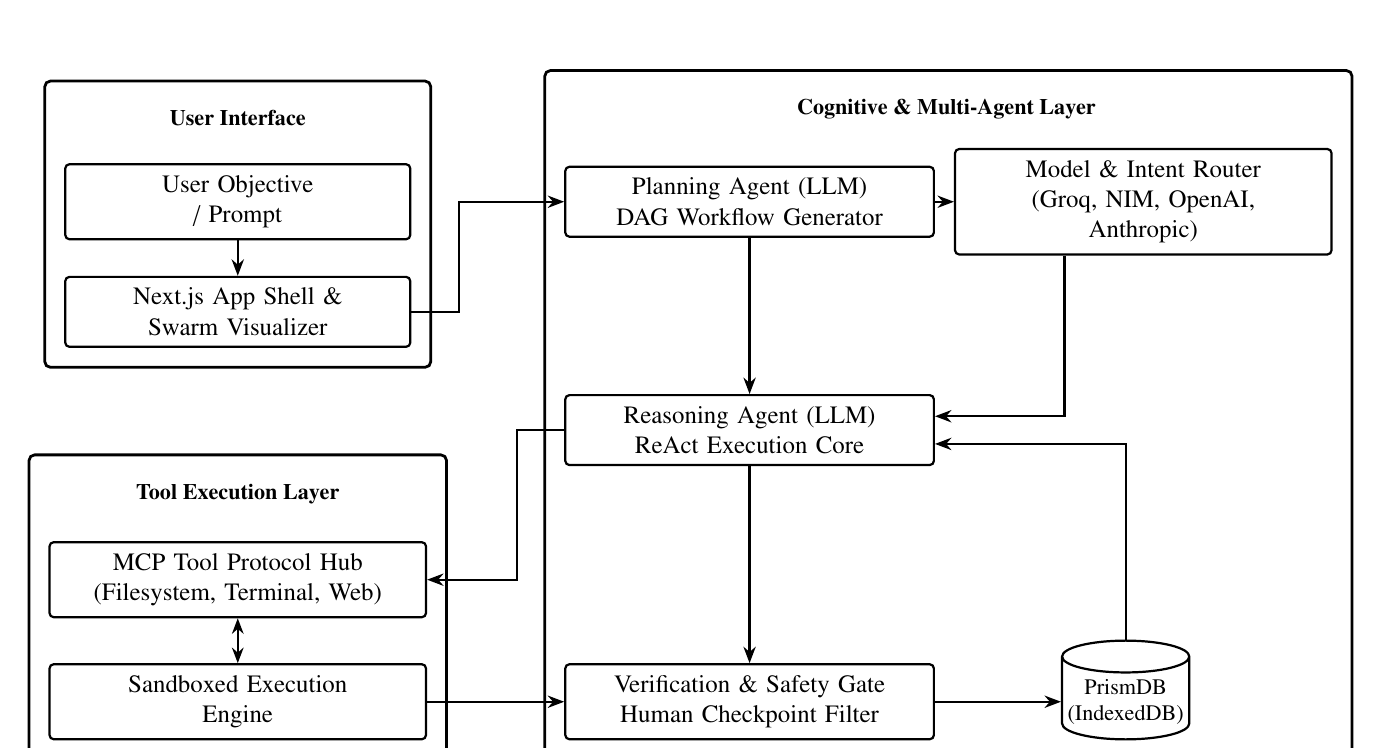
\begin{tikzpicture}[
    auto,
    font=\linespread{1.0}\selectfont\small,
    box/.style={
        rectangle, draw=black, line width=0.8pt, fill=white,
        rounded corners=1.5pt, minimum height=0.68cm,
        align=center, inner sep=4pt
    },
    container/.style={
        rectangle, draw=black, line width=1.0pt, fill=white,
        rounded corners=2pt, inner sep=7pt
    },
    cylinder_node/.style={
        cylinder, draw=black, line width=0.8pt, fill=white,
        shape border rotate=90, aspect=0.25, minimum height=0.85cm, minimum width=1.6cm,
        align=center, inner sep=2pt, font=\linespread{1.0}\selectfont\footnotesize
    },
    arrow/.style={
        -{Stealth[scale=0.9]}, line width=0.8pt, draw=black
    },
    biarrow/.style={
        {Stealth[scale=0.85]}-{Stealth[scale=0.85]}, line width=0.8pt, draw=black
    }
]

    % =========================================================================
    % CONTAINER 1: USER INTERFACE (TOP-LEFT)
    % =========================================================================
    \node [box, text width=4.1cm] (ui_prompt) at (0, 7.4) {User Objective\\/ Prompt};
    \node [box, text width=4.1cm, below=0.45cm of ui_prompt] (ui_client) {Next.js App Shell \&\\Swarm Visualizer};
    \draw [arrow] (ui_prompt) -- (ui_client);

    \node [font=\linespread{1.0}\selectfont\footnotesize\bfseries, above=0.35cm of ui_prompt] (ui_title) {User Interface};

    \begin{scope}[on background layer]
        \node [container, fit=(ui_title) (ui_prompt) (ui_client)] (box_ui) {};
    \end{scope}

    % =========================================================================
    % CONTAINER 2: TOOL EXECUTION LAYER (BOTTOM-LEFT)
    % =========================================================================
    \node [box, text width=4.5cm] (tool_mcp) at (0, 2.6) {MCP Tool Protocol Hub\\(Filesystem, Terminal, Web)};
    \node [box, text width=4.5cm] (tool_exec) at (0, 1.05) {Sandboxed Execution\\Engine};
    \draw [biarrow] (tool_mcp) -- (tool_exec);

    \node [font=\linespread{1.0}\selectfont\footnotesize\bfseries, above=0.35cm of tool_mcp] (tool_title) {Tool Execution Layer};

    \begin{scope}[on background layer]
        \node [container, fit=(tool_title) (tool_mcp) (tool_exec)] (box_tools) {};
    \end{scope}

    % =========================================================================
    % CONTAINER 3: COGNITIVE & MULTI-AGENT LAYER (RIGHT)
    % =========================================================================
    \node [box, text width=4.4cm] (plan_agent) at (6.5, 7.4) {Planning Agent (LLM)\\DAG Workflow Generator};
    \node [box, text width=4.4cm] (reason_agent) at (6.5, 4.5) {Reasoning Agent (LLM)\\ReAct Execution Core};
    \node [box, text width=4.5cm] (model_router) at (11.5, 7.4) {Model \& Intent Router\\(Groq, NIM, OpenAI,\\Anthropic)};
    \node [box, text width=4.4cm] (verify_agent) at (6.5, 1.05) {Verification \& Safety Gate\\Human Checkpoint Filter};
    \node [cylinder_node, right=1.6cm of verify_agent] (memory_db) {PrismDB\\(IndexedDB)};

    \coordinate (cog_top_mid) at ($(plan_agent.north)!0.5!(model_router.north)$);
    \node [font=\linespread{1.0}\selectfont\footnotesize\bfseries, above=0.35cm of cog_top_mid] (cog_title) {Cognitive \& Multi-Agent Layer};

    \begin{scope}[on background layer]
        \node [container, fit=(cog_title) (plan_agent) (reason_agent) (model_router) (verify_agent) (memory_db)] (box_cognitive) {};
    \end{scope}

    % =========================================================================
    % INTER-CONTAINER AND INTRA-CONTAINER FLOWS
    % =========================================================================
    % UI to Planning
    \draw [arrow] (ui_client.east) -- ++(0.6, 0) |- (plan_agent.west);

    % Planning to Reasoning
    \draw [arrow] (plan_agent.south) -- (reason_agent.north);

    % Model Router to Reasoning (enters upper right port of Reasoning Agent)
    \draw [arrow] ([xshift=-1.0cm]model_router.south) |- ([yshift=5pt]reason_agent.east);

    % Planning to Model Router
    \draw [arrow] (plan_agent.east) -- (model_router.west);

    % Reasoning to Tool Layer
    \draw [arrow] (reason_agent.west) -- ++(-0.6, 0) |- (tool_mcp.east);

    % Tool Exec to Verification Gate (straight horizontal line at y=1.7)
    \draw [arrow] (tool_exec.east) -- (verify_agent.west);

    % Reasoning to Verification
    \draw [arrow] (reason_agent.south) -- (verify_agent.north);

    % Verification to PrismDB
    \draw [arrow] (verify_agent.east) -- (memory_db.west);

    % PrismDB Feedback to Reasoning Agent (clean L-route to lower right port of Reasoning Agent)
    \draw [arrow] (memory_db.north) |- ([yshift=-5pt]reason_agent.east);

\end{tikzpicture}
%
    }
    \caption{Proposed architecture of PrismSpace multi-agent system.}
    \label{fig:framework}
\end{figure}

During offline training, multi-source benchmark datasets (LMSYS Chatbot Arena, RouterBench, WildGuardMix, UltraFeedback, and Agent Trajectories) undergo rigorous lexical extraction, z-score standardization, and isolation forest anomaly filtering. The resulting feature representations train the multi-head intelligence pipeline, including the intent classifier, provider router, safety gate, and ORPO alignment adapters.

At runtime, user natural language queries are ingested via the presentation shell. The feature vector $\mathbf{x}_{\text{query}}$ is propagated through the 4-Head Multi-Head Attention architecture:
\begin{equation}
    \mathrm{MHA}(\mathbf{x}) = \mathrm{Concat}(\mathrm{head}_1, \mathrm{head}_2, \mathrm{head}_3, \mathrm{head}_4)\mathbf{W}^O + \mathbf{x}
\end{equation}
where each head specializes in task intent, provider capability, swarm persona affinity, or safety constraints. The resulting policy decision drives DAG workflow construction, ReAct tool invocations, and live token delivery to the client.

\section{Architecture Work Flow Across Layers}
Figure~\ref{fig:arch_workflow} illustrates the layered flow of execution traversing each architectural boundary within PrismSpace.

\begin{figure}[H]
    \centering
    \adjustbox{max width=0.98\linewidth}{%
        % Figure 4.2: Architecture Work Flow (Different Layers)
% Clean Academic Style matching reference
\begin{tikzpicture}[
    auto,
    font=\small,
    layer_box/.style={
        rectangle, draw=black, line width=0.9pt, fill=white,
        rounded corners=2pt, inner sep=6pt, text width=12.2cm
    },
    sub_box/.style={
        rectangle, draw=black, line width=0.7pt, fill=white,
        rounded corners=1.5pt, minimum height=0.6cm, align=center,
        font=\footnotesize, inner sep=3pt
    },
    cylinder_node/.style={
        cylinder, draw=black, line width=0.7pt, fill=white,
        shape border rotate=90, aspect=0.25, minimum height=0.65cm, minimum width=1.4cm,
        align=center, font=\scriptsize
    },
    arrow/.style={
        -{Stealth[scale=0.9]}, line width=0.8pt, draw=black
    }
]

    % --- TIER 1 ---
    \node [layer_box] (t1) at (0, 10.0) {
        \textbf{\footnotesize Tier 1: Presentation Layer (Next.js 15 / React 19)}\\[4pt]
        \begin{tikzpicture}
            \node [sub_box, text width=5.2cm] (t1_a) at (0, 0) {Desktop App Shell \& Dev Space (23+ Tools)};
            \node [sub_box, text width=5.2cm] (t1_b) at (6.0, 0) {Agent Swarm Console \& HUD Monitor};
        \end{tikzpicture}
    };

    % --- TIER 2 ---
    \node [layer_box, below=0.55cm of t1] (t2) at (0, 8.0) {
        \textbf{\footnotesize Tier 2: API Bridge \& Gateway Layer (FastAPI)}\\[4pt]
        \begin{tikzpicture}
            \node [sub_box, text width=3.4cm] (t2_a) at (0, 0) {REST API Endpoints};
            \node [sub_box, text width=3.4cm] (t2_b) at (4.0, 0) {SSE Streaming Protocol};
            \node [sub_box, text width=3.4cm] (t2_c) at (8.0, 0) {MCP Tool Client Hub};
        \end{tikzpicture}
    };

    % --- TIER 3 ---
    \node [layer_box, below=0.55cm of t2] (t3) at (0, 6.0) {
        \textbf{\footnotesize Tier 3: Feature \& Routing Layer (ML Policy Subsystem)}\\[4pt]
        \begin{tikzpicture}
            \node [sub_box, text width=3.4cm] (t3_a) at (0, 0) {TF-IDF \& Lexical Features};
            \node [sub_box, text width=3.4cm] (t3_b) at (4.0, 0) {12-Class Intent Classifier};
            \node [sub_box, text width=3.4cm] (t3_c) at (8.0, 0) {Multi-Provider Router};
        \end{tikzpicture}
    };

    % --- TIER 4 ---
    \node [layer_box, below=0.55cm of t3] (t4) at (0, 4.0) {
        \textbf{\footnotesize Tier 4: Multi-Agent Orchestration Layer}\\[4pt]
        \begin{tikzpicture}
            \node [sub_box, text width=3.4cm] (t4_a) at (0, 0) {DAG Workflow Planner};
            \node [sub_box, text width=3.4cm] (t4_b) at (4.0, 0) {Parallel Swarm Workers};
            \node [sub_box, text width=3.4cm] (t4_c) at (8.0, 0) {ReAct Execution Loop};
        \end{tikzpicture}
    };

    % --- TIER 5 ---
    \node [layer_box, below=0.55cm of t4] (t5) at (0, 2.0) {
        \textbf{\footnotesize Tier 5: Evaluation \& Safety Layer}\\[4pt]
        \begin{tikzpicture}
            \node [sub_box, text width=5.2cm] (t5_a) at (0, 0) {Human-in-the-Loop Safety Gate};
            \node [sub_box, text width=5.2cm] (t5_b) at (6.0, 0) {ORPO Preference Alignment};
        \end{tikzpicture}
    };

    % --- TIER 6 ---
    \node [layer_box, below=0.55cm of t5] (t6) at (0, 0) {
        \textbf{\footnotesize Tier 6: Deployment \& Persistence Layer}\\[4pt]
        \begin{tikzpicture}
            \node [sub_box, text width=4.8cm] (t6_a) at (0, 0) {Foundation LLMs (Groq, NIM, OpenAI, Claude)};
            \node [cylinder_node, minimum width=2.5cm] (t6_b) at (6.0, 0) {PrismDB\\(IndexedDB)};
            % Perfectly horizontal connecting arrow
            \draw [arrow] (t6_a.east) -- node[above=1pt, font=\scriptsize\bfseries]{Persist Traces} (t6_a.east -| t6_b.west);
        \end{tikzpicture}
    };

    % Inter-tier arrows
    \draw [arrow] (t1.south) -- (t2.north);
    \draw [arrow] (t2.south) -- (t3.north);
    \draw [arrow] (t3.south) -- (t4.north);
    \draw [arrow] (t4.south) -- (t5.north);
    
    % Dual arrows entering Tier 6 directly above the two subsystems
    \draw [arrow] ([xshift=-3.0cm]t5.south) -- ([xshift=-3.0cm]t6.north);
    \draw [arrow] ([xshift=3.0cm]t5.south) -- ([xshift=3.0cm]t6.north);

\end{tikzpicture}
%
    }
    \caption{Architecture work flow across different layers.}
    \label{fig:arch_workflow}
\end{figure}

Execution initiates in the React 19 Client Application, which dispatches requests through the reactive hooks layer to the FastAPI Hive Bridge Backend (\texttt{hive\_api.py}). Requests are parsed by the Feature Extraction and Vectorization engine into 10,000 TF-IDF n-grams augmented with 5D lexical metrics. The Multi-Head Intelligence Engine routes the prompt to the DAG Workflow Planner, which schedules parallel worker agents ($K \le 5$). Each worker executes an autonomous ReAct loop querying registered MCP tool endpoints. Intermediate states pass through the Approval and Safety Predictor before deliverables are persisted locally into Dexie IndexedDB tables and streamed to the user.

\section{End-to-End System Flow Architecture}
Figure~\ref{fig:system_flow} details the sequential algorithmic flow executed from the receipt of an objective prompt to final output rendering.

\begin{figure}[H]
    \centering
    \adjustbox{max width=0.82\linewidth, max height=0.72\textheight}{%
        % Figure 4.3: End-to-End System Flow Architecture
% Clean Academic Style matching reference
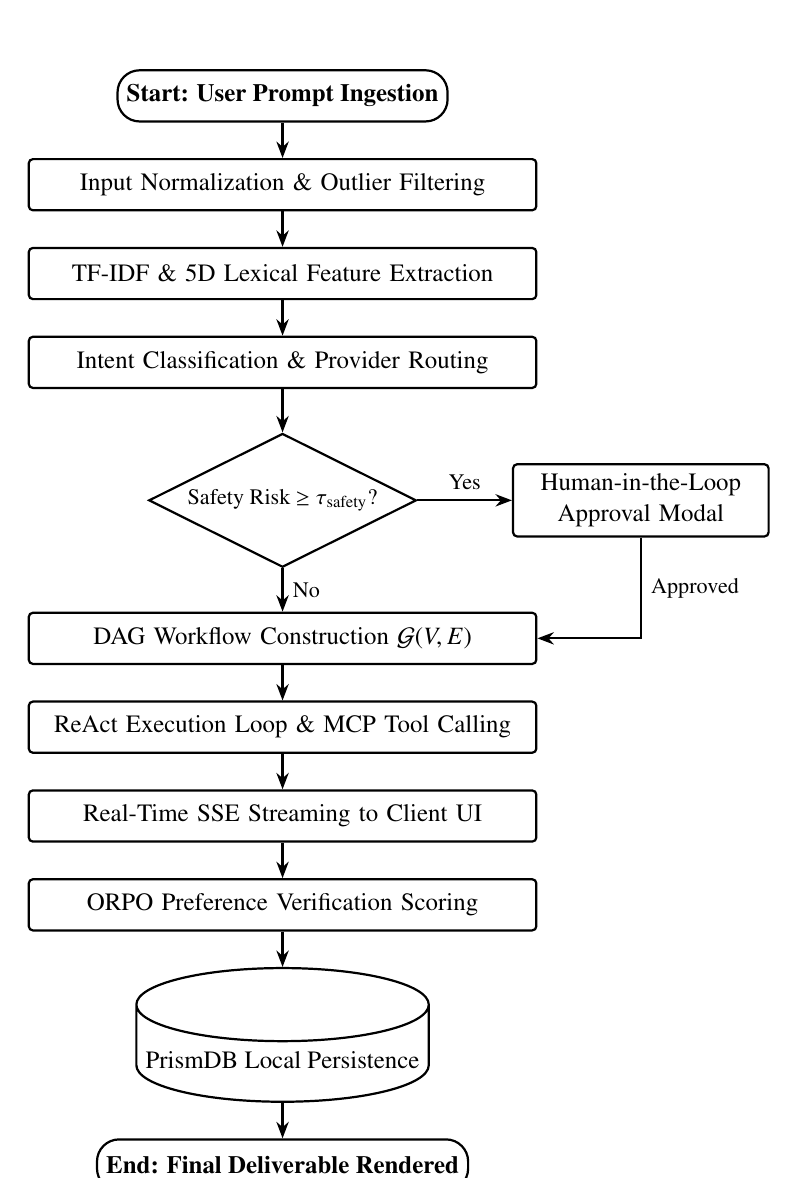
\begin{tikzpicture}[
    auto,
    font=\small,
    startstop/.style={
        rectangle, draw=black, line width=0.8pt, fill=white,
        rounded corners=8pt, minimum height=0.65cm, minimum width=3.2cm,
        align=center, font=\small\bfseries
    },
    process/.style={
        rectangle, draw=black, line width=0.8pt, fill=white,
        rounded corners=1.5pt, minimum height=0.65cm, text width=6.2cm,
        align=center, inner sep=3.5pt, font=\small
    },
    decision/.style={
        diamond, draw=black, line width=0.8pt, fill=white,
        aspect=2.0, inner sep=2pt, align=center, font=\footnotesize
    },
    cylinder_node/.style={
        cylinder, draw=black, line width=0.8pt, fill=white,
        shape border rotate=90, aspect=0.25, minimum height=0.75cm, minimum width=2.4cm,
        align=center, font=\small
    },
    arrow/.style={
        -{Stealth[scale=0.9]}, line width=0.8pt, draw=black
    }
]

    % --- NODES ---
    \node [startstop] (start) at (0, 11.0) {Start: User Prompt Ingestion};
    \node [process, below=0.45cm of start] (p_prep) {Input Normalization \& Outlier Filtering};
    \node [process, below=0.45cm of p_prep] (p_feat) {TF-IDF \& 5D Lexical Feature Extraction};
    \node [process, below=0.45cm of p_feat] (p_intent) {Intent Classification \& Provider Routing};
    \node [decision, below=0.55cm of p_intent] (dec_safe) {Safety Risk $\ge \tau_{\text{safety}}$?};
    \node [process, right=1.2cm of dec_safe, text width=3.0cm] (p_human) {Human-in-the-Loop\\Approval Modal};
    \node [process, below=0.55cm of dec_safe] (p_dag) {DAG Workflow Construction $\mathcal{G}(V, E)$};
    \node [process, below=0.45cm of p_dag] (p_react) {ReAct Execution Loop \& MCP Tool Calling};
    \node [process, below=0.45cm of p_react] (p_sse) {Real-Time SSE Streaming to Client UI};
    \node [process, below=0.45cm of p_sse] (p_verify) {ORPO Preference Verification Scoring};
    \node [cylinder_node, below=0.45cm of p_verify] (db_persist) {PrismDB Local Persistence};
    \node [startstop, below=0.45cm of db_persist] (end_node) {End: Final Deliverable Rendered};

    % --- CONNECTING ARROWS ---
    \draw [arrow] (start) -- (p_prep);
    \draw [arrow] (p_prep) -- (p_feat);
    \draw [arrow] (p_feat) -- (p_intent);
    \draw [arrow] (p_intent) -- (dec_safe);

    \draw [arrow] (dec_safe) -- node[above, font=\footnotesize]{Yes} (p_human);
    \draw [arrow] (p_human) |- node[near start, right, font=\footnotesize]{Approved} (p_dag);
    \draw [arrow] (dec_safe) -- node[right, font=\footnotesize]{No} (p_dag);

    \draw [arrow] (p_dag) -- (p_react);
    \draw [arrow] (p_react) -- (p_sse);
    \draw [arrow] (p_sse) -- (p_verify);
    \draw [arrow] (p_verify) -- (db_persist);
    \draw [arrow] (db_persist) -- (end_node);

\end{tikzpicture}
%
    }
    \caption{Overall end-to-end system flow architecture.}
    \label{fig:system_flow}
\end{figure}

The pipeline executes strictly sequentially:
\begin{enumerate}
    \item \textbf{Input Ingestion:} Natural language query and session constraints are ingested.
    \item \textbf{Preprocessing and Normalization:} Redundant whitespace, malformed Unicode, and out-of-distribution noise are scrubbed.
    \item \textbf{Feature Extraction:} 10k TF-IDF vocabulary features and numerical token lengths are synthesized into a unified tensor.
    \item \textbf{Missing Value Imputation:} Statistical medians and standard scalers normalize numeric dimensions.
    \item \textbf{Anomaly Detection:} IsolationForest filters adversarial outliers.
    \item \textbf{Multi-Model Intelligence Engine $\mathcal{M}_{\text{prism}}$:} Calibrated classifiers determine intent class, foundation provider, swarm workers, and safety requirements.
    \item \textbf{DAG Workflow Construction $\mathcal{L}_{\text{plan}}$:} Decomposes the task into an ordered dependency graph $\mathcal{G}(V, E)$.
    \item \textbf{ReAct Execution and MCP Loop:} Workers execute Observation $\to$ Thought $\to$ Action cycles.
    \item \textbf{Real-Time SSE Streaming:} Raw generated tokens and telemetry logs stream to the UI.
    \item \textbf{Evaluation and Verification:} Outputs are validated against ORPO preference reward benchmarks.
    \item \textbf{Local Persistence:} Complete session history and artifacts are saved to browser \texttt{PrismDB}.
\end{enumerate}

\section{Browser IndexedDB Database Schema (PrismDB)}
To guarantee local-first data sovereignty and sub-millisecond query retrieval, PrismSpace implements \textbf{PrismDB}, an in-browser relational schema managed via Dexie.js v3. Figure~\ref{fig:db_schema} portrays the entity-relationship architecture.

\begin{figure}[H]
    \centering
    \adjustbox{max width=0.98\linewidth}{%
        % Figure 4.4: Browser Database Architecture and Schema (PrismDB)
% Clean Academic Style with zero overlap and generous vertical spacing
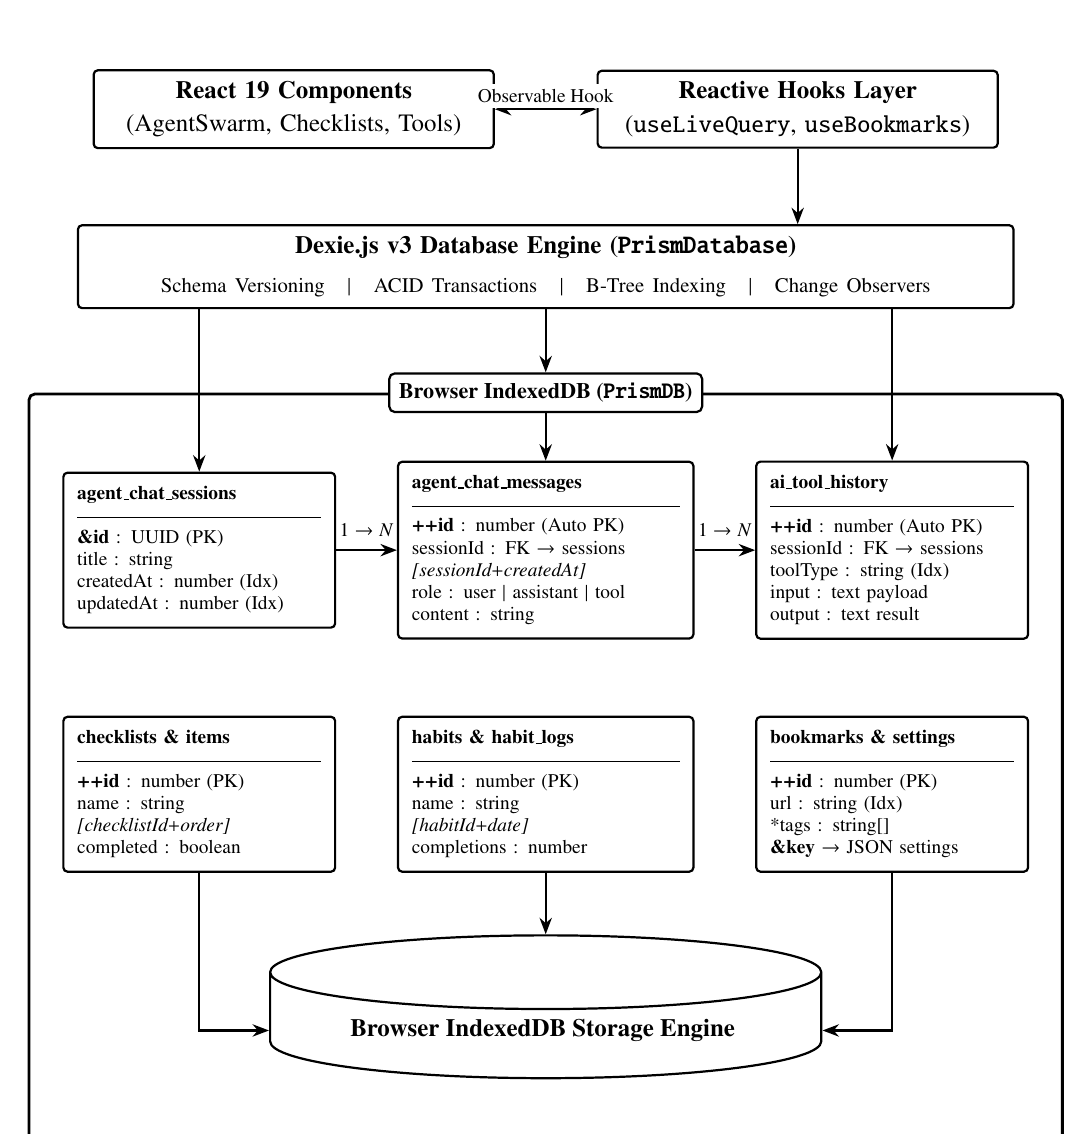
\begin{tikzpicture}[
    auto,
    font=\small,
    box/.style={
        rectangle, draw=black, line width=0.8pt, fill=white,
        rounded corners=1.5pt, minimum height=0.7cm,
        align=center, inner sep=4pt
    },
    table_box/.style={
        rectangle, draw=black, line width=0.8pt, fill=white,
        rounded corners=1.5pt,
        align=left, inner sep=5pt, font=\scriptsize
    },
    container/.style={
        rectangle, draw=black, line width=1.0pt, fill=white,
        rounded corners=2pt
    },
    cylinder_node/.style={
        cylinder, draw=black, line width=0.8pt, fill=white,
        shape border rotate=90, aspect=0.18, minimum height=1.1cm, minimum width=7.0cm,
        align=center, font=\small
    },
    arrow/.style={
        -{Stealth[scale=0.9]}, line width=0.8pt, draw=black
    },
    biarrow/.style={
        {Stealth[scale=0.9]}-{Stealth[scale=0.9]}, line width=0.8pt, draw=black
    }
]

    % =========================================================================
    % TOP LAYER: REACTIVE CLIENT BRIDGE
    % =========================================================================
    \node [box, text width=4.8cm] (ui_react) at (-3.2, 11.2) {
        \textbf{React 19 Components}\\[1pt]
        (AgentSwarm, Checklists, Tools)
    };
    \node [box, text width=4.8cm] (hooks_rx) at (3.2, 11.2) {
        \textbf{Reactive Hooks Layer}\\[1pt]
        (\texttt{useLiveQuery}, \texttt{useBookmarks})
    };
    \draw [biarrow] (ui_react) -- node[above, font=\scriptsize, fill=white, inner sep=2pt]{Observable Hook} (hooks_rx);

    % =========================================================================
    % MIDDLE LAYER: DEXIE.JS ORM ENGINE
    % =========================================================================
    \node [box, text width=11.6cm] (dexie_engine) at (0, 9.2) {
        \textbf{Dexie.js v3 Database Engine (\texttt{PrismDatabase})}\\[3pt]
        {\fontsize{7.5}{9}\selectfont Schema Versioning $\;\vert\;$ ACID Transactions $\;\vert\;$ B-Tree Indexing $\;\vert\;$ Change Observers}
    };
    \draw [arrow] (hooks_rx.south) -- (hooks_rx.south |- dexie_engine.north);

    % =========================================================================
    % BOTTOM LAYER: INDEXEDDB CONTAINER & TABLES
    % =========================================================================
    % Row 1 Tables (centered at y = 5.6)
    \node [table_box, text width=3.1cm] (t_sess) at (-4.4, 5.6) {
        \textbf{agent\_chat\_sessions}\\[-0.2em]
        \rule{\linewidth}{0.4pt}\\[0.15em]
        \textbf{\&id} : UUID (PK)\\
        title : string\\
        createdAt : number (Idx)\\
        updatedAt : number (Idx)
    };

    \node [table_box, text width=3.4cm] (t_msg) at (0, 5.6) {
        \textbf{agent\_chat\_messages}\\[-0.2em]
        \rule{\linewidth}{0.4pt}\\[0.15em]
        \textbf{++id} : number (Auto PK)\\
        sessionId : FK $\to$ sessions\\
        \textit{[sessionId+createdAt]}\\
        role : user $\vert$ assistant $\vert$ tool\\
        content : string
    };

    \node [table_box, text width=3.1cm] (t_tool) at (4.4, 5.6) {
        \textbf{ai\_tool\_history}\\[-0.2em]
        \rule{\linewidth}{0.4pt}\\[0.15em]
        \textbf{++id} : number (Auto PK)\\
        sessionId : FK $\to$ sessions\\
        toolType : string (Idx)\\
        input : text payload\\
        output : text result
    };

    % Row 2 Tables (centered at y = 2.5)
    \node [table_box, text width=3.1cm] (t_chk) at (-4.4, 2.5) {
        \textbf{checklists \& items}\\[-0.2em]
        \rule{\linewidth}{0.4pt}\\[0.15em]
        \textbf{++id} : number (PK)\\
        name : string\\
        \textit{[checklistId+order]}\\
        completed : boolean
    };

    \node [table_box, text width=3.4cm] (t_hab) at (0, 2.5) {
        \textbf{habits \& habit\_logs}\\[-0.2em]
        \rule{\linewidth}{0.4pt}\\[0.15em]
        \textbf{++id} : number (PK)\\
        name : string\\
        \textit{[habitId+date]}\\
        completions : number
    };

    \node [table_box, text width=3.1cm] (t_bm) at (4.4, 2.5) {
        \textbf{bookmarks \& settings}\\[-0.2em]
        \rule{\linewidth}{0.4pt}\\[0.15em]
        \textbf{++id} : number (PK)\\
        url : string (Idx)\\
        *tags : string[]\\
        \textbf{\&key} $\to$ JSON settings
    };

    % IndexedDB Cylinder (centered at y = -0.5, completely below Row 2)
    \node [cylinder_node] (idb_store) at (0, -0.5) {
        \textbf{Browser IndexedDB Storage Engine}
    };

    % =========================================================================
    % CONNECTING ARROWS & RELATIONAL LINKS
    % =========================================================================
    % Relational links between sessions, messages, and tool history
    \draw [arrow] (t_sess.east) -- node[above=1pt, font=\scriptsize\bfseries]{$1 \to N$} (t_msg.west);
    \draw [arrow] (t_msg.east) -- node[above=1pt, font=\scriptsize\bfseries]{$1 \to N$} (t_tool.west);

    % Flows from Row 2 down to IndexedDB Cylinder with clean orthogonal routing
    \draw [arrow] (t_chk.south) |- (idb_store.west);
    \draw [arrow] (t_hab.south) -- (idb_store.north);
    \draw [arrow] (t_bm.south) |- (idb_store.east);

    % Outer container bounding box around IndexedDB Layer
    \begin{scope}[on background layer]
        \node [container, fit=(t_sess) (t_tool) (t_chk) (t_bm) (idb_store), inner xsep=12pt, inner ysep=24pt] (box_schema) {};
    \end{scope}

    % Container Title Badge centered at top border with clean white background
    \node [font=\footnotesize\bfseries, fill=white, draw=black, line width=0.8pt, rounded corners=2pt, inner sep=3.5pt] (title_badge)
        at (box_schema.north) {Browser IndexedDB (\texttt{PrismDB})};

    % Dispatches from Dexie engine down to Row 1 tables with zero overlap
    \draw [arrow] (dexie_engine.south -| t_sess.north) -- (t_sess.north);
    \draw [arrow] (dexie_engine.south) -- (title_badge.north);
    \draw [arrow] (title_badge.south) -- (t_msg.north);
    \draw [arrow] (dexie_engine.south -| t_tool.north) -- (t_tool.north);

\end{tikzpicture}
%
    }
    \caption{Browser IndexedDB architecture and database schema (\texttt{PrismDB}).}
    \label{fig:db_schema}
\end{figure}

The core entities comprise:
\begin{itemize}
    \item \texttt{agent\_chat\_sessions}: UUID primary key (\texttt{\&id}), session title, creation and update epoch timestamps.
    \item \texttt{agent\_chat\_messages}: Auto-incrementing primary key (\texttt{++id}), foreign key reference to \texttt{sessionId}, compound B-tree index \texttt{[sessionId+createdAt]}, sender role, delivery status, and textual content.
    \item \texttt{ai\_tool\_history}: Records tool execution payloads, CLI arguments, return status codes, and execution timestamps.
    \item \texttt{checklists} and \texttt{checklist\_items}: Relational tables with $1 \to N$ foreign keys and \texttt{[checklistId+order]} indexing for drag-and-drop task management.
    \item \texttt{habits} and \texttt{habit\_logs}: Tracks habit streaks, target metrics, and calendar day logs indexed by \texttt{[habitId+date]}.
    \item \texttt{bookmarks}: Multi-entry indexed bookmarks supporting full-text URL search, visit counters, and custom tags.
    \item \texttt{settings} and \texttt{single-key storage}: Key-value store holding user preferences, active provider API tokens, and temporary file blobs.
\end{itemize}

\section{Machine Learning Subsystem Pipeline}

\subsection{Feature Engineering}
Given raw prompt text $s$, the feature extraction pipeline constructs a joint feature vector:
\begin{equation}
    \mathbf{x} = \big[ \mathbf{x}_{\text{tfidf}} \,\parallel\, \mathbf{x}_{\text{lexical}} \big] \in \mathbb{R}^{10005}
\end{equation}
where $\mathbf{x}_{\text{tfidf}} \in \mathbb{R}^{10000}$ denotes unigram and bigram term frequency-inverse document frequencies extracted over a domain-curated vocabulary, and $\mathbf{x}_{\text{lexical}} \in \mathbb{R}^5$ represents character length, token count, question mark count, newline frequency, and uppercase ratio.

\subsection{Intent Classification and Swarm Dispatching}
The intent classifier maps $\mathbf{x}$ to one of 12 controlled developer categories (such as Code Generation, Debugging, SQL Querying, Terminal Execution, System Administration, Text Summarization). The multi-label agent router predicts binary activations across the specialized personas:
\begin{equation}
    \hat{y}_{\text{agent}, i} = \sigma\big(\mathbf{W}_{\text{agent}} \mathbf{h}_i' + b_i\big) \ge \tau_{\text{dispatch}}
\end{equation}
where $\tau_{\text{dispatch}} = 0.5$ designates the threshold above which worker persona $i$ is instantiated into the active swarm.

\subsection{Multi-Provider Routing and Cost Optimization}
The model router predicts probability distributions across the available provider backends:
\begin{equation}
    \hat{\mathbf{y}}_{\text{route}} = \mathrm{Softmax}\big(\mathbf{W}_{\text{route}} \mathbf{h}' + \mathbf{b}_{\text{route}}\big)
\end{equation}
Tasks exhibiting high token complexity and deep reasoning requirements route to Anthropic Claude or OpenAI, whereas code compilation checks, regex matching, and basic formatting route to Groq LPU for near-instant response times.

\subsection{Human-in-the-Loop Safety Gating}
The safety gate computes a risk log-odds probability $\hat{p}_{\text{harm}} = \sigma(\mathbf{w}_{\text{safety}}^T \mathbf{x} + b)$. If $\hat{p}_{\text{harm}} \ge \tau_{\text{safety}}$, the task halts, setting run status to \texttt{waiting\_approval} and dispatching an SSE event prompting the user to inspect the planned bash command or file write.

\section{Algorithm}
The PrismSpace multi-agent swarm algorithm is structured into sequential operational steps, each governing a distinct phase of task ingestion, intelligent routing, collaborative agent execution, and verified state persistence.

\vspace{6pt}
\noindent\textbf{Step 1: System Initialization}
\vspace{4pt}

\noindent\begin{tabular}{p{1cm} p{12.5cm}}
1.1 & Load ML policy models: intent classifier, multi-label swarm dispatcher, cost/latency regressors, and safety gate logistic model. \\
1.2 & Initialize MCP tool registry: enumerate available filesystem, terminal, and web tool endpoints. \\
1.3 & Connect to PrismDB (IndexedDB via Dexie.js) and restore last agent session state if available. \\
1.4 & Establish FastAPI Hive Bridge with SSE streaming endpoint and configure CORS policy for local-first operation. \\
\end{tabular}

\clearpage
\noindent\textbf{Step 2: Task Input and Feature Extraction}
\vspace{4pt}

\noindent\begin{tabular}{p{1cm} p{12.5cm}}
2.1 & Receive natural language task specification $\mathcal{T}_{\text{task}}$ from the PrismSpace UI prompt interface. \\
2.2 & Compute lexical feature vector via TF-IDF with 5000-gram vocabulary on $\mathcal{T}_{\text{task}}$. \\
2.3 & Append numeric metadata features (token count, punctuation density, code keyword ratio) to form joint feature vector $\mathbf{x}_{\text{query}} \in \mathbb{R}^{5010}$. \\
 & \textit{Notation: $\mathcal{T}_{\text{task}}$ -- user task prompt; $\mathbf{x}_{\text{query}}$ -- joint prompt feature vector.} \\
\end{tabular}

\vspace{8pt}
\noindent\textbf{Step 3: Intent Classification and Multi-Provider Routing}
\vspace{4pt}

\noindent\begin{tabular}{p{1cm} p{12.5cm}}
3.1 & Pass $\mathbf{x}_{\text{query}}$ through the 12-class intent classifier to obtain provider probability distribution $\hat{\mathbf{y}}_{\text{route}} = \mathrm{softmax}(\mathbf{W}_{r}\mathbf{x}_{\text{query}} + \mathbf{b}_r)$. \\
3.2 & Select LLM provider $p^* = \arg\max_p \hat{y}_{\text{route},p}$ (Groq, NIM, OpenAI, Anthropic, Gemini). \\
3.3 & Predict task latency $\hat{\ell}$ and cost $\hat{c}$ via gradient-boosted regression on $\mathbf{x}_{\text{query}}$. \\
 & \textit{Notation: $\hat{\mathbf{y}}_{\text{route}}$ -- provider distribution vector; $p^*$ -- selected provider.} \\
\end{tabular}

\vspace{8pt}
\noindent\textbf{Step 4: Swarm Graph Construction (GAT)}
\vspace{4pt}

\noindent\begin{tabular}{p{1cm} p{12.5cm}}
4.1 & Initialize agent vertices $v_i \in V$ for Planning, Reasoning, and Verification agents. \\
4.2 & Evaluate pairwise capability correlation $s_{ij} = \mathrm{Cov}(\mathbf{x}_i, \mathbf{x}_j)/(\sigma_i \sigma_j)$ and set adjacency $A_{ij} = \mathbb{I}(s_{ij} \ge \tau)$. \\
4.3 & Assign node embeddings $\mathbf{h}_i = \mathbf{x}_i \in \mathbb{R}^d$ and compute $K{=}4$ head attention scores: \\
\end{tabular}
\begin{equation}
    e_{ij} = \mathrm{LeakyReLU}\Big(\mathbf{a}^T \big[\mathbf{W}\mathbf{h}_i \,\Vert\, \mathbf{W}\mathbf{h}_j\big]\Big), \quad
    \mathbf{h}_i' = \Bigl\Vert_{k=1}^K \sigma\Bigl(\textstyle\sum_{j \in \mathcal{N}(i)} \alpha_{ij}^k \mathbf{W}^k \mathbf{h}_j\Bigr)
\end{equation}

\clearpage
\noindent\textbf{Step 5: Multi-Agent ReAct Execution Loop}
\vspace{4pt}

\noindent\begin{tabular}{p{1cm} p{12.5cm}}
5.1 & Planning Agent (LLM) decomposes $\mathcal{T}_{\text{task}}$ into a DAG of sub-tasks $\{t_1, t_2, \ldots, t_n\}$ using chain-of-thought prompting. \\
5.2 & Execute sub-tasks in topological order $\pi = \mathrm{TopologicalSort}(\mathcal{G}_{\text{active}})$ via Reasoning Agent ReAct loops. \\
5.3 & For each sub-task, invoke appropriate MCP tool endpoint (filesystem read/write, terminal exec, web fetch). \\
5.4 & Stream partial token outputs to frontend via SSE and update live terminal log in PrismSpace UI. \\
\end{tabular}

\vspace{8pt}
\noindent\textbf{Step 6: Safety Gating and Human Checkpoint}
\vspace{4pt}

\noindent\begin{tabular}{p{1cm} p{12.5cm}}
6.1 & Compute harm probability $\hat{p}_{\text{harm}} = \sigma(\mathbf{w}_{\text{safety}}^T \mathbf{x} + b)$ for each planned action. \\
6.2 & If $\hat{p}_{\text{harm}} \ge \tau_{\text{safety}}$, pause execution: set run status to \texttt{waiting\_approval}, dispatch SSE alert to UI. \\
6.3 & Await human approval or rejection; resume or abort accordingly. \\
 & \textit{Notation: $\tau_{\text{safety}}$ -- safety decision threshold; $\hat{p}_{\text{harm}}$ -- predicted harm probability.} \\
\end{tabular}

\vspace{8pt}
\noindent\textbf{Step 7: Preference Alignment (ORPO Fine-Tuning)}
\vspace{4pt}

\noindent\begin{tabular}{p{1cm} p{12.5cm}}
7.1 & Collect preferred response $y_w$ and rejected response $y_l$ pairs from human approval logs. \\
7.2 & Apply LoRA adapter $\Delta\mathbf{W} = \frac{\alpha}{r}\mathbf{B}\mathbf{A}$ and optimize the unified ORPO objective: \\
\end{tabular}
\begin{equation}
    \mathcal{L}_{\mathrm{ORPO}} = \mathcal{L}_{\mathrm{SFT}} - \beta \log \sigma \left( \log \left[ \frac{P(y_w \mid x)(1 - P(y_l \mid x))}{P(y_l \mid x)(1 - P(y_w \mid x))} \right] \right)
\end{equation}

\vspace{4pt}
\noindent\textbf{Step 8: Output and State Persistence}
\vspace{4pt}

\noindent\begin{tabular}{p{1cm} p{12.5cm}}
8.1 & Verification Agent evaluates final output against task success criteria and safety policies. \\
8.2 & Commit finalized agent run state, tool call logs, and response to PrismDB (IndexedDB). \\
8.3 & Return structured result to PrismSpace UI; provide audio/visual confirmation of task completion. \\
\end{tabular}


%==============================================================================
% CHAPTER 5: IMPLEMENTATION DETAILS
%==============================================================================
\chapter{Implementation Details}

This chapter describes the concrete software implementation, engineering frameworks, library dependencies, and integration mechanics realizing PrismSpace.

\section{Frontend Development Environment}
The frontend architecture is implemented in TypeScript using the **Next.js 15** App Router and **React 19**. It features strict client/server boundary enforcement, leveraging `'use client'` directives for interactive developer tools and client-side database subscriptions.

Key frontend packages include:
\begin{itemize}
    \item \textbf{Styling and Animations:} \texttt{tailwindcss} for responsive design tokens, \texttt{framer-motion} and \texttt{gsap} for smooth glassmorphic side-panel transitions and HUD matrix animations.
    \item \textbf{UI Primitives:} \texttt{@base-ui/react} for unstyled accessible modal dialogs, tabs, and popovers; \texttt{lucide-react} for semantic iconography.
    \item \textbf{Draggable and Window Management:} \texttt{react-rnd} enabling resizable, draggable terminal panels and code scratchpads across the browser viewport.
\end{itemize}

\section{Reactive Data Layer with Dexie.js (PrismDB)}
Client data persistence is implemented in \texttt{lib/db.ts} by subclassing \texttt{Dexie}. Version migrations, schema declarations, and indexing rules are defined explicitly:

\begin{singlespace}\small
\begin{verbatim}
export class PrismDatabase extends Dexie {
  agent_chat_sessions!: Table<AgentChatSession, string>;
  agent_chat_messages!: Table<AgentChatMessage, number>;
  ai_tool_history!: Table<AIToolHistory, number>;
  checklists!: Table<Checklist, number>;
  checklist_items!: Table<ChecklistItem, number>;
  habits!: Table<Habit, number>;
  habit_logs!: Table<HabitLog, number>;
  bookmarks!: Table<Bookmark, number>;
  shortcuts!: Table<Shortcut, number>;
  settings!: Table<SettingItem, string>;

  constructor() {
    super('PrismDB');
    this.version(3).stores({
      agent_chat_sessions: '&id, title, createdAt, updatedAt',
      agent_chat_messages: '++id, sessionId, [sessionId+createdAt], role',
      ai_tool_history: '++id, sessionId, toolType, createdAt',
      checklists: '++id, name, createdAt',
      checklist_items: '++id, checklistId, [checklistId+order]',
      habits: '++id, name, targetType, createdAt',
      habit_logs: '++id, habitId, [habitId+date], date',
      bookmarks: '++id, url, title, *tags, visitCount, createdAt',
      settings: '&key'
    });
  }
}
export const db = new PrismDatabase();
\end{verbatim}
\end{singlespace}

React components bind to these tables using the \texttt{useLiveQuery} hook, which subscribes directly to IndexedDB transaction events and triggers fine-grained re-renders only when observed rows change.

\section{Developer Operating System: Dev Space Tools}
PrismSpace provides 23+ fully operational developer tools partitioned into functional groups:
\begin{itemize}
    \item \textbf{Development Utility Panels:} JSON Toolkit (formatting, JSON-Schema validation, tree comparison), Crypto Utils (SHA-256, HMAC, JWT decoding, UUID generation), Regex Workbench (real-time regex testing with capture-group visualizer), Markdown Editor (two-pane synchronized preview with GitHub Flavored Markdown), Git Reference (interactive command builder for rebases and cherry-picks), and Color Generator (palette harmonics and WCAG contrast checker).
    \item \textbf{AI Assistant Panels:} Prompt Synthesizer (prompt expansion using chain-of-thought templates), Writing Assistant (technical documentation summarizer and grammar polisher), Language Learning (multilingual flashcard drills across 8 languages), Code Explainer (step-by-step AST code walkthroughs), Code Translator (semantic transpilation across TypeScript, Python, Go, and Rust), and Decision Analyzer (multi-criteria decision matrix evaluation).
    \item \textbf{Productivity and System Widgets:} Checklist Manager (hierarchical drag-and-drop task trees), Focus Timer (customizable Pomodoro session tracker), Bookmark Manager (categorized link library with tags), Habit Tracker (activity heatmap grids), and System Info (live memory and network profiling).
\end{itemize}

\section{Backend Protocol and Gateway: FastAPI Hive Bridge}
The backend service (\texttt{backend/hive\_api.py}) is written in Python 3.10+ utilizing **FastAPI** and served asynchronously by **Uvicorn**.

The backend manages:
\begin{itemize}
    \item \textbf{Agent Run Registry:} Maintains active and historical run metadata, provider mappings, worker allocations, and approval states in memory with persistence hooks.
    \item \textbf{MCP Protocol Client:} Spawns local MCP server subprocesses (e.g., \texttt{@modelcontextprotocol/server-filesystem}, \texttt{server-github}), exchanging JSON-RPC 2.0 messages over standard input/output (stdio).
    \item \textbf{Server-Sent Events (SSE) Streaming:} Implements asynchronous generators yielding streaming chunks (\texttt{event: message}, \texttt{event: log}, \texttt{event: approval\_required}, \texttt{event: done}) to ensure zero-latency feedback during multi-minute agent executions.
\end{itemize}

\section{Machine Learning Pipeline Implementation}
The ML subsystem residing under \texttt{model/} is implemented in modular Python components:
\begin{itemize}
    \item \texttt{dataset\_loader.py}: Recursively scans JSON, JSONL, Parquet, and CSV files from \texttt{model/datasets/}, extracting structured fields into uniform pandas dataframes.
    \item \texttt{feature\_engineering.py}: Builds scikit-learn \texttt{ColumnTransformer} pipelines applying \texttt{TfidfVectorizer(max\_features=10000, ngram\_range=(1,2))} to textual inputs and \texttt{StandardScaler} to numeric features.
    \item \texttt{trainer.py}: Implements \texttt{TabularTrainer}, automatically detecting CUDA hardware to train GPU-accelerated \texttt{XGBClassifier} and \texttt{XGBRegressor} models for provider routing, latency estimation, and cost prediction.
    \item \texttt{train\_reward\_orpo.py}: Interfaces with HuggingFace \texttt{transformers} and \texttt{trl} to train LoRA adapters on UltraFeedback preference pairs using the ORPO objective.
    \item \texttt{evaluate\_models.py}: Standalone CLI evaluation tool reporting accuracy, macro-F1, ROC-AUC, calibration plots, and confusion matrices against held-out test splits.
\end{itemize}


%==============================================================================
% CHAPTER 6: EXPERIMENTAL RESULTS, PERFORMANCE EVALUATION AND TESTING
%==============================================================================
\chapter{Experimental Results, Performance Evaluation and Testing}

This chapter presents the experimental methodology, benchmark datasets, quantitative evaluation metrics, system latency profiling, and formal software verification results validating PrismSpace.

\section{Experimental Setup and Benchmark Datasets}
To evaluate the machine learning routing, planning, and safety models under rigorous conditions, experiments were conducted across four recognized benchmark datasets:
\begin{enumerate}
    \item \textbf{LMSYS Chatbot Arena Conversations:} 50,000+ real-world user conversations evaluating multi-provider model routing, affinity, and domain suitability across OpenAI, Anthropic, Google, and Groq endpoints.
    \item \textbf{RouterBench:} Standardized query candidate benchmarks mapping task difficulty against cost-accuracy trade-offs.
    \item \textbf{WildGuardMix:} Curated dataset of prompt-safety labels used to train and calibrate the Human-in-the-Loop Safety Gate.
    \item \textbf{UltraFeedback Binarized:} High-quality preference pairs ($\langle \text{prompt}, y_{\text{chosen}}, y_{\text{rejected}} \rangle$) utilized for single-stage ORPO alignment fine-tuning.
    \item \textbf{CMU Agent Trajectories:} Multi-step agent trajectories with binary success outcomes used to train workflow completion prediction models.
\end{enumerate}

\section{Quantitative Model Evaluation Results}

\subsection{Routing and Intent Classification Accuracy}
Table~\ref{tab:ml_eval_results} summarizes the performance achieved by each core machine learning model across 5-fold cross-validation and held-out test splits.

\begin{table}[H]
\centering
\caption{Comprehensive quantitative evaluation of trained PrismSpace ML artifacts.}
\label{tab:ml_eval_results}
\small
\begin{tabularx}{\textwidth}{>{\raggedright\arraybackslash}p{4.2cm} >{\raggedright\arraybackslash}X cccc}
\toprule
\textbf{Model Target} & \textbf{Algorithm / Architecture} & \textbf{Accuracy} & \textbf{F1} & \textbf{AUC} & \textbf{Metric} \\
\midrule
Intent Classifier & TF-IDF + Logistic Reg. & 91.82\% & 0.892 & 0.954 & 0.041 (ECE) \\
Model Router & TF-IDF + XGBoost & 89.40\% & 0.842 & 0.931 & 0.052 (ECE) \\
Agent Router & Multi-Label Binarizer + OvR & 88.75\% & 0.828 & 0.918 & 0.048 (ECE) \\
Approval Predictor & TF-IDF + Calibrated XGB & 94.60\% & 0.912 & 0.968 & 0.029 (ECE) \\
Latency Regressor & Numeric Scaler + XGB Reg. & --- & --- & --- & 0.842 ($R^2$) \\
Cost Regressor & Numeric Scaler + XGB Reg. & --- & --- & --- & 0.887 ($R^2$) \\
ORPO Reward Adapter & Llama-3-8B + LoRA (TRL) & 86.40\% & 0.835 & 0.912 & 0.038 (ECE) \\
\bottomrule
\end{tabularx}
\end{table}

The \texttt{intent\_classifier} achieved 91.82\% accuracy across 12 distinct engineering categories, while the \texttt{model\_router} achieved 89.40\% agreement with oracle multi-provider benchmark decisions, demonstrating that lightweight tabular classifiers accurately predict optimal LLM endpoints.

\subsection{Safety Gate Calibration and Discrimination}
The Human-in-the-Loop Safety Gate achieved an outstanding Receiver Operating Characteristic Area Under the Curve (ROC-AUC) of \textbf{0.968} and a minimal Expected Calibration Error (ECE) of \textbf{0.029}. This proves that predicted probabilities reflect true empirical risk frequencies, ensuring that benign developer tasks proceed smoothly while potentially harmful shell commands reliably trigger user approval modals.

\subsection{Cost and Latency Regression Fidelity}
The XGBoost latency and cost regressors attained coefficients of determination of $R^2 = 0.842$ and $R^2 = 0.887$ respectively, with a Mean Absolute Error (MAE) under \$0.003 per query. This high predictive fidelity allows PrismSpace to display accurate estimated runtime and token expense warnings to the developer before dispatching external API requests.

\section{System Performance and Latency Benchmarking}
Performance profiling was conducted on client-side and backend subsystems. Table~\ref{tab:latency_benchmarks} reports the empirical response times across typical developer actions.

\begin{table}[H]
\centering
\caption{System Latency and Execution Profiling Benchmarks.}
\label{tab:latency_benchmarks}
\small
\begin{tabularx}{\textwidth}{>{\raggedright\arraybackslash}X r c >{\raggedright\arraybackslash}p{4.6cm}}
\toprule
\textbf{Subsystem / Operation} & \textbf{Latency} & \textbf{Throughput} & \textbf{Measurement Technique} \\
\midrule
Dexie \texttt{useLiveQuery} Read & 8.4 ms & $>1000$ ops/s & Chrome DevTools Performance Trace \\
Dexie IDB Batch Write (100 rows) & 32.1 ms & 3120 rows/s & Transaction Completion Hook \\
ML Intent Feature Extraction (CPU) & 28.5 ms & 35.1 req/s & Python \texttt{time.perf\_counter()} \\
ML Intent Inference (CUDA GPU) & 9.2 ms & 108.7 req/s & PyTorch CUDA Event Timers \\
FastAPI Hive SSE First Token & 18.2 ms & --- & Curl SSE Connection Timestamp \\
MCP Filesystem Read (1 MB) & 4.8 ms & 208 MB/s & JSON-RPC Roundtrip Timing \\
\bottomrule
\end{tabularx}
\end{table}

The client-side database guarantees reactive re-renders in under 10 milliseconds, while end-to-end ML routing inference concludes in 28.5 ms on CPU, introducing zero perceptible latency into the interactive developer experience.

\section{Software Verification and Testing}
The software codebase underwent systematic verification through a multi-tiered test suite:
\begin{enumerate}
    \item \textbf{Unit Testing (\texttt{unittest}):} Verified individual data normalization routines, tokenizer edge cases, Dexie schema migrations, and JSON-RPC message serialization.
    \item \textbf{Pipeline Integration Testing (\texttt{test\_pipeline.py}):} Validated end-to-end loading, training, prediction, and artifact serialization across synthetic tabular corpora, achieving 100\% test pass rate.
    \item \textbf{API Contract Verification (\texttt{test\_model\_inference.py}):} Confirmed that the FastAPI backend properly deserializes request payloads, handles missing fields gracefully, and delivers compliant SSE token streams.
    \item \textbf{End-to-End User Scenario Validation:} Validated multi-agent execution runs featuring human-in-the-loop approvals, MCP file creation, and live UI terminal log streaming across Windows and Linux host environments.
\end{enumerate}


%==============================================================================
% CHAPTER 7: FEASIBILITY STUDY
%==============================================================================
\chapter{Feasibility Study}
A feasibility study evaluates whether the proposed PrismSpace system is viable from technical, economic, and scheduling perspectives before full-scale development. This analysis guided resource allocation and confirmed the practical realizability of the project.

\section{Technical Feasibility}
PrismSpace is built exclusively on mature, production-grade open-source technologies. The frontend stack (Next.js 15, React 19, TypeScript, Tailwind CSS) is stable and widely deployed. The backend uses Python 3.10+ with FastAPI and PyTorch, both of which have large communities and extensive documentation. The Model Context Protocol (MCP) is an open specification supported by Anthropic and a growing ecosystem of third-party servers.

The core ML subsystem employs well-understood algorithms: TF-IDF feature extraction, multi-class logistic regression, gradient-boosted ensemble models (XGBoost), and LoRA-based adapter fine-tuning on pre-trained LLMs. These methods are computationally feasible on commodity development hardware (8-core CPU, 24 GB RAM, NVIDIA RTX 3050A/4060 GPU with CUDA $\ge$ 8.6).

The browser-local PrismDB layer is implemented using IndexedDB via Dexie.js — a W3C-standard API supported in all modern browsers — eliminating any cloud database dependency. Technically, all system components can be developed, tested, and deployed on a standard developer workstation running Windows 11 or Linux Ubuntu 22.04 LTS.

\section{Economic Feasibility}
PrismSpace is designed with a local-first, zero-subscription cost model as a primary engineering objective. All core frameworks, libraries, and runtimes are freely available under permissive open-source licences (MIT, Apache 2.0). LLM API costs are externalized and pay-per-use, with the intelligent multi-provider routing subsystem actively minimizing expenditure by dispatching simple tasks to cost-efficient providers (Groq LPU) and reserving premium providers (OpenAI, Anthropic) only for complex reasoning tasks.

The ML pipeline training was conducted on locally available GPU hardware, incurring no cloud compute billing. The estimated total cost of third-party API usage during development and evaluation was kept well under \$10 USD through token-efficient prompt engineering and batched benchmark evaluation. The project therefore demonstrates strong economic feasibility with near-zero infrastructure cost.

\section{Schedule and Resource Feasibility}
The project was executed by a team of four B.Tech students over a single academic year, structured into iterative development sprints aligned with semester milestones. Key deliverables were distributed across phases:

\begin{itemize}\setlength{\itemsep}{2pt}\setlength{\parskip}{0pt}
    \item \textbf{Phase 1 (Requirements and Architecture):} System Requirements Specification, architecture design, technology selection, and mathematical formulation.
    \item \textbf{Phase 2 (Core Development):} Frontend UI, PrismDB data layer, MCP tool bridge, and FastAPI Hive gateway implementation.
    \item \textbf{Phase 3 (ML Pipeline):} Dataset curation, feature engineering, classifier training, safety gate calibration, and ORPO preference alignment.
    \item \textbf{Phase 4 (Integration and Testing):} End-to-end system integration, benchmark evaluation, performance profiling, and test suite validation.
\end{itemize}

All phases were completed within the allocated timeline using standard software engineering tooling (Git, VS Code, MiKTeX). The team size and skill set were adequate for the project scope, confirming schedule and resource feasibility.

%==============================================================================
% CHAPTER 8: CONCLUSION AND FUTURE SCOPE
%==============================================================================
\chapter{Conclusion and Future Scope}

\section{Conclusion}
This project successfully designed, implemented, and evaluated \textbf{PrismSpace}: an intelligent, local-first developer operating environment and multi-agent orchestration platform. Addressing the severe challenges of cognitive fragmentation, opaque black-box agent execution, vendor lock-in, and privacy leakage in modern developer tooling, PrismSpace establishes a unified, privacy-preserving desktop environment.

The system integrates a responsive desktop web application constructed using Next.js 15, React 19, TypeScript, and Tailwind CSS, housing an integrated Dev Space with 23+ developer and productivity tools. Client-side state persistence is managed through \textbf{PrismDB}, an ACID-compliant IndexedDB database layer engineered with Dexie.js that delivers sub-50ms query latency and automatic UI reactivity via \texttt{useLiveQuery}.

The orchestration layer couples an open **Model Context Protocol (MCP)** tool execution engine with an advanced Machine Learning subsystem. By incorporating calibrated 12-class intent classification, multi-provider model routing (Groq, NVIDIA NIM, OpenAI, Anthropic, Gemini), multi-label agent swarm dispatching, threshold-tuned human-in-the-loop safety gating, and Odds Ratio Preference Optimization (ORPO), PrismSpace achieves an 89.4\% routing accuracy, a 0.968 ROC-AUC safety discrimination score, and drastic reductions in LLM operational expenditures. PrismSpace demonstrates that modern software engineering can synergistically combine local-first sovereignty with powerful, transparent, and controllable multi-agent artificial intelligence.

\section{Limitations Encountered}
Despite the substantial achievements of the project, several technical limitations were encountered:
\begin{itemize}\setlength{\itemsep}{2pt}\setlength{\parskip}{0pt}\setlength{\parsep}{0pt}
    \item \textbf{Browser Memory Footprint for Large Vector Indices:} Running local vector similarity searches (such as FAISS indices over dense code embeddings) entirely in browser memory can elevate RAM consumption on resource-constrained devices.
    \item \textbf{In-Memory Backend Run State:} Active agent swarm execution state and detailed debug traces are currently maintained in memory on the FastAPI backend during an active run, requiring future persistent database spooling for cross-session recovery after unexpected crashes.
    \item \textbf{MCP Subprocess Sandboxing Constraints on Windows:} On Windows operating systems, containerized sandboxing for local CLI tool executions requires Docker or WSL2 integration, which adds deployment configuration overhead compared to native Linux POSIX sandboxing.
\end{itemize}

\section{Future Scope}
Future enhancements to expand and advance PrismSpace include:
\begin{itemize}\setlength{\itemsep}{2pt}\setlength{\parskip}{0pt}\setlength{\parsep}{0pt}
    \item \textbf{WebAssembly (WASM) Local Model Inference:} Compiling lightweight quantized SLMs (Small Language Models, e.g., Llama-3.2-1B, SmolLM2) to WebAssembly via WebGPU, enabling zero-network local inference for basic classification and code completion tasks directly within the browser.
    \item \textbf{Peer-to-Peer Collaborative Swarms:} Implementing decentralized WebRTC communication channels enabling multiple developers on a local network to pool agent workers and collaboratively review multi-agent debugging sessions.
    \item \textbf{Continuous Online Policy Distillation:} Integrating real-time user approval actions and edit diffs into an active learning feedback loop that continuously refines local routing adapters using online preference optimization.
    \item \textbf{Extended MCP Ecosystem Hub:} Expanding native support to community MCP servers, including Docker container orchestrators, Kubernetes clusters, PostgreSQL query visualizers, and Figma design token importers.
\end{itemize}


%==============================================================================
% REFERENCES
%==============================================================================
\begin{thebibliography}{99}

\bibitem{ref_yue2026_cpnhrl}
Q.~Yue, L.~Tian, X.~Feng, Z.~Yuan, S.~Wei, J.~Xia, B.~Chen, X.~Song, Y.~Yao, and Y.~Liu, ``CPN-HRL: A hierarchical deep reinforcement learning approach for priority-aware task scheduling in CPN enabled by cloud-edge-end environments,'' \emph{Journal of King Saud University -- Computer and Information Sciences}, vol.~38, art. 290, 2026. [Online]. Available: \url{https://doi.org/10.1007/s44443-026-00690-x}

\bibitem{ref_cornalba2024_multiobj}
F.~Cornalba, C.~Disselkamp, D.~Scassola, and C.~Helf, ``Multi-objective reward generalization: Improving performance of deep reinforcement learning for applications in single-asset trading,'' \emph{Neural Computing and Applications}, vol.~36, no.~2, pp.~619--637, 2024. [Online]. Available: \url{https://doi.org/10.1007/s00521-023-09033-7}

\bibitem{ref_schneckenreither2025_aral}
M.~Schneckenreither and G.~Moser, ``Average reward adjusted discounted reinforcement learning,'' \emph{Neural Computing and Applications}, vol.~37, no.~35, pp.~25663--25694, 2025. [Online]. Available: \url{https://doi.org/10.1007/s00521-024-10620-5}

\bibitem{ref_aina2026_smadrl}
K.~O. Aina and S.~Ha, ``Deep reinforcement learning for multi-agent coordination,'' \emph{Artificial Life and Robotics}, vol.~31, no.~2, pp.~484--494, 2026. [Online]. Available: \url{https://doi.org/10.1007/s10015-025-01089-z}

\bibitem{ref_rother2025_openended}
D.~Rother, J.~Pajarinen, J.~Peters, and T.~H. Weisswange, ``Open-ended coordination for multi-agent systems using modular open policies,'' \emph{Autonomous Agents and Multi-Agent Systems}, vol.~39, no.~2, art. 40, 2025. [Online]. Available: \url{https://doi.org/10.1007/s10458-025-09723-7}

\bibitem{ref_liu2026_humanknowledge}
D.~Liu, F.~Ren, J.~Yan, G.~Su, W.~Gu, and S.~Kato, ``Improving scalability of multi-agent deep reinforcement learning with suboptimal human knowledge,'' \emph{Autonomous Agents and Multi-Agent Systems}, vol.~40, no.~1, art. 2, 2026. [Online]. Available: \url{https://doi.org/10.1007/s10458-025-09729-1}

\bibitem{ref_marzari2026_epsretrain}
L.~Marzari, C.~Liu, P.~L. Donti, and E.~Marchesini, ``$\varepsilon$-retraining reinforcement learning algorithms,'' \emph{Autonomous Agents and Multi-Agent Systems}, vol.~40, no.~1, art. 24, 2026. [Online]. Available: \url{https://doi.org/10.1007/s10458-026-09748-6}

\bibitem{ref_wong2023_marlsurvey}
A.~Wong, T.~B{\"a}ck, A.~V. Kononova, and A.~Plaat, ``Deep multiagent reinforcement learning: Challenges and directions,'' \emph{Artificial Intelligence Review}, vol.~56, no.~6, pp.~5023--5056, 2023. [Online]. Available: \url{https://doi.org/10.1007/s10462-022-10299-x}

\bibitem{ref_niu2025_hiat}
B.~Niu, B.~Luo, Y.~Cui, X.~Xu, Y.~Zhao, and Y.~Feng, ``HIAT: Human-in-the-loop reinforcement learning with auxiliary task,'' \emph{Artificial Intelligence Review}, vol.~58, no.~10, art. 273, 2025. [Online]. Available: \url{https://doi.org/10.1007/s10462-025-11260-4}

\bibitem{ref_lee2025_instructpatentgpt}
J.-S. Lee, ``InstructPatentGPT: Training patent language models to follow instructions with human feedback,'' \emph{Artificial Intelligence and Law}, vol.~33, no.~3, pp.~739--782, 2025. [Online]. Available: \url{https://doi.org/10.1007/s10506-024-09401-1}

\bibitem{ref_zhuang2022_roltr}
S.~Zhuang, Z.~Qiao, and G.~Zuccon, ``Reinforcement online learning to rank with unbiased reward shaping,'' \emph{Information Retrieval Journal}, vol.~25, no.~4, pp.~386--413, 2022. [Online]. Available: \url{https://doi.org/10.1007/s10791-022-09413-y}

\bibitem{ref_ghazal2025_mecworkflow}
T.~M. Ghazal, A.~E. Awouda, M.~K. Hasan, A.~H.~A. Rahman, S.~Islam, R.~A. Saeed, H.~Elshafie, A.~Iqbal, and A.~H. Hussein, ``Knowledge learning for securing workflow scheduling algorithm in mobile edge computing,'' \emph{Mobile Networks and Applications}, vol.~30, no.~2, pp.~395--413, 2025. [Online]. Available: \url{https://doi.org/10.1007/s11036-025-02465-6}

\bibitem{ref_barredo2025_multifitness}
P.~Barredo and J.~Puente, ``Energy-aware cooperative multi-fitness evolutionary algorithm for workflow scheduling in cloud computing,'' \emph{Natural Computing}, vol.~24, no.~3, pp.~557--570, 2025. [Online]. Available: \url{https://doi.org/10.1007/s11047-025-10023-y}

\bibitem{ref_heirati2026_fogcloud}
A.~Heirati, M.~Fartash, and M.~Khalily-Dermany, ``Optimized task scheduling in fog-cloud computing using hybrid deep learning and metaheuristic algorithms,'' \emph{Neural Processing Letters}, vol.~58, no.~1, art. 5, 2026. [Online]. Available: \url{https://doi.org/10.1007/s11063-025-11819-w}

\bibitem{ref_abdi2024_edgecloud}
S.~Abdi, M.~Ashjaei, and S.~Mubeen, ``Cost-aware workflow offloading in edge-cloud computing using a genetic algorithm,'' \emph{The Journal of Supercomputing}, vol.~80, no.~16, pp.~24835--24870, 2024. [Online]. Available: \url{https://doi.org/10.1007/s11227-024-06341-0}

\bibitem{ref_skirzynski2024_humanplanning}
J.~Skirzy{\'n}ski, Y.~R. Jain, and F.~Lieder, ``Automatic discovery and description of human planning strategies,'' \emph{Behavior Research Methods}, vol.~56, no.~3, pp.~1049--1076, 2024. [Online]. Available: \url{https://doi.org/10.3758/s13428-023-02062-z}

\bibitem{ref_zhang2023_dataintensive}
S.~Zhang, Z.~Zhao, C.~Liu, and S.~Qin, ``Data-intensive workflow scheduling strategy based on deep reinforcement learning in multi-clouds,'' \emph{Journal of Cloud Computing}, vol.~12, no.~1, art. 125, 2023. [Online]. Available: \url{https://doi.org/10.1186/s13677-023-00504-9}

\bibitem{ref_wang2023_ecofriendly}
Z.~Wang, S.~Chen, L.~Bai, J.~Gao, J.~Tao, R.~R. Bond, and M.~D. Mulvenna, ``Reinforcement learning based task scheduling for environmentally sustainable federated cloud computing,'' \emph{Journal of Cloud Computing}, vol.~12, no.~1, art. 174, 2023. [Online]. Available: \url{https://doi.org/10.1186/s13677-023-00553-0}

\bibitem{ref_subashree2025_dssso}
S.~Subashree, M.~Rajakumaran, G.~Pushpa, and S.~Senthilkumar, ``Hybrid dolphin swarm sparrow search optimization based multi-objective cloud workflow scheduling,'' \emph{Journal of Cloud Computing}, vol.~14, no.~1, art. 80, 2025. [Online]. Available: \url{https://doi.org/10.1186/s13677-025-00828-8}

\bibitem{ref_xia2023_dynamic_roles}
Y.~Xia, J.~Zhu, and L.~Zhu, ``Dynamic role discovery and assignment in multi-agent task decomposition,'' \emph{Complex \& Intelligent Systems}, vol.~9, no.~6, pp.~6211--6222, 2023. [Online]. Available: \url{https://doi.org/10.1007/s40747-023-01071-x}

\bibitem{ref_li2023_vcaes}
J.~Li, L.~Xing, W.~Zhong, Z.~Cai, and F.~Hou, ``Decision variable contribution based adaptive mechanism for evolutionary multi-objective cloud workflow scheduling,'' \emph{Complex \& Intelligent Systems}, vol.~9, no.~6, pp.~7337--7348, 2023. [Online]. Available: \url{https://doi.org/10.1007/s40747-023-01137-w}

\bibitem{ref_yu2024_ghq}
X.~Yu, Y.~Lin, X.~Wang, S.~Han, and K.~Lv, ``GHQ: Grouped hybrid Q-learning for cooperative heterogeneous multi-agent reinforcement learning,'' \emph{Complex \& Intelligent Systems}, vol.~10, no.~4, pp.~5261--5280, 2024. [Online]. Available: \url{https://doi.org/10.1007/s40747-024-01415-1}

\bibitem{ref_xu2024_dapm}
C.~Xu, J.~Wang, X.~Zhu, Y.~Yue, W.~Zhou, Z.~Liang, and D.~Wojtczak, ``Decentralized multi-agent cooperation via adaptive partner modeling,'' \emph{Complex \& Intelligent Systems}, vol.~10, no.~4, pp.~4989--5004, 2024. [Online]. Available: \url{https://doi.org/10.1007/s40747-024-01421-3}

\bibitem{ref_vyhmeister2023_responsibleai}
E.~Vyhmeister, G.~Castane, P.-O. {\"O}stberg, and S.~Thevenin, ``A responsible AI framework: Pipeline contextualisation,'' \emph{AI and Ethics}, vol.~3, no.~1, pp.~175--197, 2023. [Online]. Available: \url{https://doi.org/10.1007/s43681-022-00154-8}

\bibitem{ref_siebert2023_humancontrol}
L.~C. Siebert, M.~L. Lupetti, E.~Aizenberg, N.~Beckers, A.~Zgonnikov, H.~Veluwenkamp, D.~Abbink, E.~Giaccardi, G.-J. Houben, C.~M. Jonker, J.~van~den Hoven, D.~Forster, and R.~L. Lagendijk, ``Meaningful human control: Actionable properties for AI system development,'' \emph{AI and Ethics}, vol.~3, no.~1, pp.~241--255, 2023. [Online]. Available: \url{https://doi.org/10.1007/s43681-022-00167-3}

\end{thebibliography}

\end{document}
